\documentclass[12pt,notitlepage]{article}
\usepackage[utf8]{inputenc}
\usepackage{geometry}
\geometry{verbose,tmargin=1.25in,bmargin=1.25in,lmargin=1in,rmargin=1in}
\usepackage{verbatim}
\usepackage{float}
\usepackage{bm}
\usepackage{amsmath}
\usepackage{amssymb}
\usepackage{graphicx}
\usepackage{setspace}
\usepackage[authoryear]{natbib}
\usepackage{booktabs}

\onehalfspacing

\makeatletter

\usepackage{amsfonts}
\usepackage{multicol}
\usepackage{pdflscape}

\setcounter{MaxMatrixCols}{10}

\usepackage{fancyhdr}
\usepackage[utf8]{inputenc}

% This gives Roman section numbers
%\renewcommand{\thesection}{\Roman{section}} 
%\renewcommand{\thesubsection}{\thesection.\Alph{subsection}}

% This gives assumption numbers
\usepackage{amsmath}  
%\newtheorem{assumption}{Assumption}
%\newtheorem{lemma}{Lemma}

% Scalars
%\input{../input/results/scalars}

%\usepackage[latin9]{inputenc}
%\usepackage{geometry}
%\geometry{verbose,tmargin=1in,bmargin=1in,lmargin=1in,rmargin=1in}
\usepackage{float}
\usepackage{amsthm}
\usepackage{amsmath}
\usepackage{amssymb}
\usepackage{graphicx}
\usepackage{setspace}
\doublespace
\usepackage{esint}  
\usepackage[authoryear]{natbib}
\usepackage{hyperref}
\usepackage{comment}
\usepackage[normalem]{ulem}
\usepackage{array}
\usepackage{multirow}
\usepackage{float}
\usepackage{cancel}
\usepackage{enumerate}
\makeatletter
\makeatother
%\numberwithin{equation}{section} %numbering equation with section number
\usepackage{pgf,tikz}
\usepackage{mathrsfs}
\usetikzlibrary{arrows}
\usepackage[english]{babel}


\theoremstyle{plain}
\newtheorem{theorem}{\protect\theoremname}
\theoremstyle{plain}
\newtheorem*{theorem*}{\protect\theoremname}
\theoremstyle{definition}
\newtheorem{definition}{\protect\definitionname}
\theoremstyle{definition}
\newtheorem*{definition*}{\protect\definitionname}
\theoremstyle{assumption}
\newtheorem{assumption}{\protect\assumptionname}
\theoremstyle{plain}
\newtheorem{corollary}{\protect\corollaryname}
\theoremstyle{plain}
\newtheorem{lemma}{\protect\lemmaname}
\theoremstyle{plain}
\newtheorem{proposition}{\protect\propositionname}
\theoremstyle{plain}
\newtheorem{conjecture}{\protect\conjecturename}
\theoremstyle{definition}%%%12/28/2019
\newtheorem{remark}{\protect\remarkname}
\theoremstyle{plain}
\newtheorem{claim}{\protect\claimname}
\theoremstyle{plain}
\newtheorem{fact}{\protect\factname}
\theoremstyle{plain}
\newtheorem{result}{\protect\resultname}
\theoremstyle{plain}
\newtheorem{observation}{\protect\observationname}

\providecommand{\claimname}{Claim}
\providecommand{\conjecturename}{Conjecture}
\providecommand{\corollaryname}{Corollary}
\providecommand{\lemmaname}{Lemma}
\providecommand{\definitionname}{Definition}
\providecommand{\assumptionname}{Assumption}
\providecommand{\examplename}{Example}
\providecommand{\factname}{Fact}
\providecommand{\propositionname}{Proposition}
\providecommand{\remarkname}{Remark}
\providecommand{\theoremname}{Theorem}
\providecommand{\resultname}{Result}
\providecommand{\observationname}{Observation}


\usepackage{subcaption}
\makeatletter
\renewcommand{\fnum@figure}{Figure \thefigure}
\makeatother

%%%%%%%%%%OWN%%%%%%%%%%%%%%%%%%%%%%%%%%%%%%%%%%%%%%%%%%%%%%%%%%%%%%%%%%%%%%%%%%%%%%%%%%%%%%%%%%%%%%%%%%%%%%%%%%%%%%%%%%%%%%%
\usepackage[font=footnotesize]{caption} 

\usepackage{physics}
\usepackage{enumitem}
\usepackage{pgfplots}
\usepackage{mathtools}
\newcommand*\diff{\mathop{}\!\mathrm{d}}

\DeclareMathOperator*{\argmax}{arg\,max}
\DeclareMathOperator*{\argmin}{arg\,min}
\DeclareMathOperator{\supp}{Supp}
\DeclareMathOperator{\proj}{Proj}
\DeclareMathOperator{\prob}{Pr}


\usepackage{istgame}
\usetikzlibrary{shapes.geometric,arrows}

\usepackage{xcolor}
\usepackage{wrapfig}

\newcommand{\pdfcolor}{blue!85!black}
\hypersetup{colorlinks=true,linkcolor=\pdfcolor,citecolor=\pdfcolor,urlcolor=\pdfcolor}


\usepackage{bm}

\makeatother

\begin{document}
\title{Sharing Opinions in the Shadow of AI}

\author{Elliott Ash, Yichuan Lou, and Lena Song\thanks{Ash: ETH Zurich, ashe@ethz.ch. Lou: University of Tokyo, yichuanlou@e.u-tokyo.ac.jp.
Song: University of Illinois Urbana-Champaign, lenasong@illinois.edu. We thank John List and Marta Serra-Garcia and seminar and conference participants at ETHZ, UIUC, UCSD, UChicago, Advances in Field Experiments, and Stockholm Online Political Influence and Misinformation Conference for helpful comments. 
We thank Sahil Adane and Amin Rahmati for excellent research assistance. The study
was approved by Institutional Review Boards at University of Illinois
Urbana-Champaign (IRB24-0588). This experiment was registered in the American Economic Association Registry for randomized controlled trials under trial number AEARCTR-0013548 (\url{https://www.socialscienceregistry.org/trials/13548}). }}
\maketitle
\begin{abstract}
\singlespacing \noindent We study how the presence of artificial intelligence (AI) agents affects human content production in online interactions. We develop a theoretical framework in which a human sender caring about social image and exposure risk composes messages for a human receiver. We derive conditions under which the presence of AI co-senders encourages or discourages human participation in content production. We show that concerns about exposure risk reduce participation, and that the presence of AI can increase participation by mitigating these concerns. We test the model's predictions using an online survey experiment. Consistent with the theory, the effect of AI presence on participation depends on whether the sender's identity may be disclosed. When identity disclosure is possible, the presence of AI increases participation, consistent with mitigated exposure-risk concerns. In contrast, when senders remain anonymous, AI presence has little effect on participation. Our findings contribute to ongoing debates about the societal impact of AI by showing that AI can reshape content production not only through machine-generated content, but also by altering the reputational incentives of human contributors.

\vspace{12pt}

\noindent Keywords: Artificial Intelligence, Signaling, Social Image, Experiments

\end{abstract}


\medskip{}

\onehalfspacing 

\newpage{}

\section{Introduction} 

Digital communication increasingly takes place in mixed environments where human users interact alongside automated agents. While simple bots have long existed online \citep{Varol_Ferrara_Davis_Menczer_Flammini_2017}, recent advances in generative AI have made automated participation far more human-like. These systems can now produce fluent and contextually appropriate text that readers often struggle to distinguish from human writing \citep[e.g.][]{brown2020language}. As a result, the online audience can no longer assume that every post, comment, or reply reflects the views and intentions of a human speaker.

That change matters because the decision to contribute online is often shaped by social incentives. Participation in online discussions can generate social rewards when it signals conviction, engagement, or intrinsic motivation to contribute \citep{aridor2024economics}. At the same time, speaking in public forums can carry reputational costs when statements become associated with an individual’s identity and are subject to scrutiny or criticism \citep{BenabouTirole:06,BursztynJensen:17,braghieri2024political}. When generative AI becomes a plausible source of online messages, participation no longer clearly signals that a contribution comes from a human author \citep[e.g.][]{cui2025signaling,galdin2025making}. This ambiguity may weaken the reputational value of contributing, but it may also reduce the perceived exposure that comes from having one's views attributed to a specific person.

These opposing forces raise an important question: how does the presence of generative AI affect human participation in online discussions? To address this question, we study how the presence of generative AI alters human content production in online social interactions. When AI becomes a plausible source of online messages, participation becomes a noisier signal of human authorship, weakening both the reputational rewards and the exposure risks associated with contributing. Whether AI discourages or encourages human participation therefore depends on how individuals trade off image rewards against exposure risk when deciding whether to speak.

We first develop a theoretical framework for social interactions, building on the signaling approach of \citet{BenabouTirole:06}. In our framework, human agents choose whether to participate in content production. Participation yields intrinsic utility but also generates belief-based payoffs that depend on how observers interpret the action. A first novel ingredient in our model is that these belief-based payoffs involve both an expected benefit via social image and an expected cost from the risk of exposure when sensitive views are linked to personal identity \citep{BursztynJensen:17}. Exposure risk reflects an important aspect of online interactions: participation is not always tied to real identity, but when it is, expressing views may expose individuals to criticism or other reputational consequences. The effect of being identified on participation depends on the relative importance of these two payoffs. 

A second new ingredient in the model is the co-presence of generative AI bots. Because bots can take the same observable participation action as humans, their presence makes participation a noisy signal of human identity. By diluting the inference that a participant is human, AI can weaken reputational incentives to contribute, but it can also reduce exposure concerns by loosening the perceived connection between content and identity. Which force dominates depends on the relative strength of image concerns and sensitivity to exposure.

To test these ideas, we conduct a survey experiment with university students in which participants decide whether to produce opinion content in exchange for a monetary payment. Participants are offered compensation (about \$12.50 USD) to answer a survey and compose a short post on how they and other students in Zurich can contribute to combating climate change, which may be shown to other students at their university. Participants who do not complete the writing task forgo the payment. We experimentally vary two features of the environment. First, we vary whether messages are pooled exclusively with other human-written posts or with a mix that includes generative AI–generated content. Second, we vary whether participants' identity may be disclosed to readers or whether they remain anonymous. This design isolates how AI presence and identity disclosure jointly shape incentives to contribute content.

We find that when student identities are disclosed, there is a significant reduction in participation in the writing task. Compared to the anonymous condition (where participation is close to 100\%), students in the identified condition are much more likely to leave the study and forego the payment. In our conceptual framework, that is consistent with the expected costs of exposing one's views on a sensitive topic outweighing the expected benefits of signaling a virtuous view on that topic. 

Next we consider the additional effect of AI co-senders. Strikingly, the presence of AI substantially mitigates the effects of identification on participation. When participants are identifiable, introducing AI increases completion rates and the likelihood of producing a meaningful post. By contrast, when participants remain anonymous, AI has no effect on participation. These patterns are strongest among participants with higher sensitivity to exposure and among women. Together, the results support the model's central mechanism: AI reshapes human engagement not by replacing human expression, but by weakening the perceived link between authored content and personal identity.

These theoretical and empirical results add to the growing body of literature on content production in the digital world. A growing literature studies the incentives that drive content production in online environments. Prior work shows that participation is shaped by a combination of intrinsic motivations, reputation concerns, attention, and social feedback \citep{aridor2024economics}. Recent work has also examined how automated responses affect participation. For example, \citet{srinivasan2023} shows that randomly allocating AI-generated replies to Reddit posts increases subsequent content production by users. Rather than studying how AI responses affect human activity, our paper examines how the presence of AI content creators changes the incentives of human producers themselves.

A related literature studies how generative AI affects the informational content of communication and performance signals. Because AI can produce high-quality text at low cost, observers may find it harder to infer underlying ability or effort from written outputs \citep{cowgill2024cheapen,cui2025signaling,galdin2025making}. A related strand of work examines how AI tools affect productivity and behavior in workplace settings \citep{noy2023experimental,brynjolfsson2024generative,almog2025barriers}, and how individuals respond when AI systems evaluate or monitor their work \citep{almoggauriotpage2025oversight,almoglippmanmartin2026judges}.\footnote{A related experimental literature studies how individuals behave differently when interacting with machines rather than humans \citep{chugunova2022we}. For example, people are more likely to cheat when interacting with machines \citep{marechal2020}, and allowing AI-generated promises changes trust dynamics in communication games \citep{bogliacino2023}.} While this literature primarily focuses on how AI changes the quality of produced output or the adoption of AI tools, our paper studies how the presence of AI changes the incentives for humans to participate in communication in the first place.

The paper also relates to the literature on social image and reputational incentives. A growing body of empirical work shows that individuals adjust their actions when those actions are observable and can influence how they are perceived by others \citep{BursztynJensen:17}. In digital environments, reputational incentives have been shown to influence behaviors such as political expression, misinformation sharing, and protest participation on social media \citep{enikolopov2020social,guriev2026,braghieri2024political}.\footnote{A broader empirical literature documents the role of social image concerns in shaping behavior across a range of settings, including workplace effort \citep{MasMoretti:09}, voting and political participation \citep{Funk:10,DellaVigna:17}, and charitable giving and prosocial actions \citep{DellaVigna:12,Ashraf:14}.} Our paper contributes to this literature by examining how advances in generative AI change the reputational environment of online communication by weakening the inference that an observed contribution reflects the views of a human author.

Our model adds to the theoretical literature on social image. Following \citet{BenabouTirole:06}, we adopt a signaling approach to social interactions in which individuals care about how they are perceived by others and therefore behave strategically to influence those perceptions. Our model has three novel ingredients. First, we study an environment in which humans coexist with automated agents that can take the same costly participation action, thereby diluting the informational content of participation and weakening the inference that a participant is human. Second, in addition to social image concerns, an individual's indirect utility also reflects exposure risk when authorship is linked to personal identity. In our setting, this exposure cost arises only when participation is attributed to a human author whose identity may be revealed. Third, unlike \citet{BenabouTirole:06}, we assume that abstention from the task carries neither reputational costs nor benefits, reflecting the fact that users on social media can always opt out without generating reputation-related payoffs.

The rest of the paper is structured as follows. Section 2 outlines
the theoretical framework. Section 3 describes and reports the results of the experiment. Section 4 concludes. 

\section{Theoretical Framework}\label{sec:theoretical framework}

This section develops a simple signaling framework to formalize how the presence of AI may affect human participation in online content production. The model highlights a tension between two forces. Participation can generate social image benefits when it signals intrinsic motivation to contribute, but it may also impose exposure costs when authored content can be linked to a person's identity. The presence of generative AI weakens the inference that a participant is human, thereby diluting both image rewards and exposure risks. The framework clarifies the conditions under which AI discourages or instead encourages human participation, and it guides the empirical predictions tested in the experiment.

Subsection \ref{subsec:model} presents the model and characterizes the equilibrium. Subsection \ref{subsec:predictions} derives the comparative statics that guide the empirical predictions tested in the experiment.

\subsection{Model} \label{subsec:model}

The model builds on the large theoretical and empirical literature that explains prosocial behavior as the outcome of intrinsic motivation, participation costs, and social image concerns. We extend this framework to an environment in which human agents coexist with automated agents whose actions may be observationally indistinguishable from human behavior. Two features are central. First, we allow non-human agents---generative AI and rule-based bots---to take the same participation action as humans (e.g., posting content or contributing messages). Second, in addition to standard social image concerns, we incorporate exposure concerns: conditional on being perceived as human, participation may entail an additional utility cost arising from potential identity disclosure. Together, these features capture how the presence of bot agents reshapes the incentives for human participation in prosocial activities.


\paragraph{Agents, types, and actions.} There is a continuum of agents. Each agent belongs to one of three identity groups: humans ($h$), generative-AI bots ($g$), and rule-based bots ($r$). For example, in an online discussion forum, humans are verified account holders, generative-AI bots are LLM-powered accounts producing fluent, contextually varied posts, and rule-based bots are scripted accounts posting templated messages. Let $(p_h,p_g,p_r)$ denote the population shares, with $p_h+p_g+p_r=1$.

Human agents have private type $v\in[\underline{v},\overline{v}]$ with $\underline{v}> 0$, interpreted as intrinsic motivation to participate. The prior distribution of $v$ is $F$, which has a continuous density $f$ with full support on $[\underline{v},\overline{v}]$. Each human agent makes a binary decision: $a\in \{0,1\}$, where $a=1$ represents participation and $a=0$ represents abstention. Participation entails a cost $c>0$. If a human agent abstains, she receives outside option $u_0\in\mathbb R$. If she participates, she receives \textit{direct utility} $v-c$ plus an indirect payoff that depends on how observers interpret participation.

Bots do not have private types. A generative-AI bot chooses $a=1$ with probability $\alpha\in(0,1)$ and takes a detectable action $a_g\notin\{0,1\}$ with probability $1-\alpha$. A rule-based bot always takes a detectable action $a_r\notin\{0,1\}$. Detectable actions are interpreted as non-human and thus never pooled with human participation---for example, a CAPTCHA failure, a platform-issued bot label, or a posting pattern readily identifiable as non-human.


\paragraph{Information, beliefs, and payoffs.} Observers see the realized action. If they observe a detectable action ($a_g$ or $a_r$), they assign probability one to the agent being a bot. The relevant inference problem therefore arises after observing participation $a=1$, which can be generated by humans and, with probability $\alpha$, by generative-AI bots. Let $\prob(h\mid a=1)$ denote the perceived probability that a participant is human. 

For human agents, participation has reputational consequences beyond its direct payoff. As in \cite{BenabouTirole:06}, participation can serve as a signal of prosocial motivation and thus generate social approval: observers who attribute the action to a human may update upward their assessment of the agent's intrinsic motivation. At the same time, participation may lead to identity disclosure, giving rise to a reputational cost. In our setting, both the approval benefit and the exposure cost are belief-based and thus are relevant only insofar as the participant is believed to be human; if participation is attributed to a non-human sender, neither prosocial credit nor exposure risk is at stake.


Let $\mu\ge 0$ denote the strength of image concerns and $\gamma\ge 0$ the strength of exposure risk concerns. The \textit{indirect/reputational utility} from participation for a human is
\begin{align*}
    \prob(h\mid a=1)\big(\mu \mathbb{E}[v\mid a=1] - \gamma\big).
\end{align*}
Intuitively, participation yields an image benefit from being perceived as prosocial but may also trigger exposure costs. Both effects are scaled by the likelihood that the participant is human. Thus, a human of type $v$ who participates obtains total utility
\begin{align*}
    v-c+\prob(h\mid a=1)\big(\mu \mathbb{E}[v\mid a=1] - \gamma\big).
\end{align*}

If instead the human agent abstains, she receives her outside option with value $u_0$, which is independent of beliefs and carries no endogenous reputational payoff. Our key modeling assumption is therefore that indirect payoffs arising from social image and exposure risk are attached only to participation, not to abstention. In \cite{BenabouTirole:06}, both actions generate reputational consequences, with ``honor" from participating and ``stigma" from abstaining. By contrast, in our setting abstention is interpreted as \emph{non-observation}: if an agent does not post, there is no observable content for the audience to evaluate and therefore no reputational inference about the agent. Consequently, only participation generates image benefits and exposure risk.

Using the payoffs derived above for participation and abstention, a human agent participates whenever
\[
v-c+\prob(h\mid a=1)\big(\mu \mathbb{E}[v\mid a=1] - \gamma\big)\geq u_0.
\]


\paragraph{Timing and equilibrium.} Nature first draws the agent's identity. If the agent is human, nature further draws the human agent's type $v$. The agent then chooses an action. Observers update beliefs using Bayes' rule whenever possible. A (Perfect Bayesian) equilibrium consists of (i) a strategy for each human type and (ii) beliefs over identity and, conditional on being human, over type $v$, such that strategies are optimal given beliefs and beliefs are Bayes-consistent on path.\footnote{Unlike in standard signaling games, off-the-equilibrium-path beliefs are immaterial in this environment and therefore need not be refined \`a la \cite{ChoKreps:87}. When full participation ($a=1$) occurs on path, a human agent's deviation to $a=0$ does not generate any image or exposure payoff, so beliefs (over both identity and value $v$) following $a=0$ are payoff-irrelevant. When no participation ($a=0$) occurs on path, the action $a=1$ remains on path because Gen-AI bots take $a=1$ with positive probability. In this case, following a deviation by a human agent, $\prob(h\mid a=1)$ remains zero, so the indirect payoff is again null.}


Because only participation can be pooled between humans and generative-AI bots, the equilibrium characterization is conveniently expressed in terms of the participation cutoff $v^*$ and the posterior probability that a participant is human. In any cutoff equilibrium with threshold $v^*$, human agents participate if and only if $v\geq v^*$, so $\mathbb{E}[v\mid a=1] = \mathbb{E}[v\mid v\geq v^*]$. Define the \textit{net image-exposure surplus} conditional on being perceived as human by $T(v^*)\triangleq \mu \mathbb{E}[v\mid v\geq v^*] - \gamma$. Let $\rho\triangleq\frac{p_g}{p_h+p_g}$ denote the share of generative-AI bots among agents whose actions may be confounded with human participation. Under a cutoff strategy at $v^*$, Bayes' rule implies that the posterior probability a participant is human is $\pi(v^*)\triangleq \prob(h\mid a=1) =  \frac{(1-\rho)(1-F(v^*))}{\rho \alpha + (1-\rho)(1-F(v^*))}$. Given a candidate cutoff $v^*$, a human type $v$ prefers participation if and only if $v-c+\pi(v^*)T(v^*)\geq u_0$. 


Define the operator $\Phi(v)\triangleq v - c + \pi(v)T(v)$, where $\pi(v)T(v)$ captures the indirect payoff from participation through prosocial image and exposure channels. We impose $\Phi'(v)>0$ on $(\underline v,\overline v)$ to ensure a unique stable equilibrium.\footnote{See Appendix \ref{appendix:theoretical framework} for a detailed discussion of equilibrium stability and uniqueness.}

\begin{proposition}\label{prop:equilibrium}
    Suppose $\Phi'(v)>0$ on $(\underline v,\overline v)$. There is a unique equilibrium:
    \begin{itemize}
        \item[(i)] If $u_0\in(\Phi(\underline{v}),\Phi(\overline{v}))$, then $a=0$ for $v\in[\underline{v},v^*)$ and $a=1$ for $(v^*,\overline{v}]$, where $v^*$ uniquely solves $\Phi(v^*)=u_0$.
        \item[(ii)] If $u_0\geq\Phi(\overline{v})$, then $a=0$ for all $v\in[\underline{v},\overline{v}]$.
        \item[(iii)] If $u_0\leq \Phi(\underline{v})$, then $a=1$ for all $v\in[\underline{v},\overline{v}]$.
    \end{itemize}
\end{proposition}


\subsection{Key Predictions} \label{subsec:predictions}

In an interior equilibrium, the cutoff $v^*$ satisfies
\[
u_0=v^*-c+\pi(v^*)T(v^*)
\]
where
$\pi(v^*) = \frac{(1-\rho)(1-F(v^*))}{\rho \alpha + (1-\rho)(1-F(v^*))}$ is the posterior probability that a participant is human, and $T(v^*)=\mu \mathbb{E}[v\mid v\geq v^*] - \gamma$ is the net image-exposure surplus conditional on being perceived as human. The product $\pi(v^*)T(v^*)$ highlights that the indirect payoff from participation depends on two components: how likely participation is to be attributed to a human, and how valuable it is to be perceived as human. Within $T(v^*)$, we refer to $\mu \mathbb{E}[v\mid v\geq v^*]$ as the ``honor"  conferred by participation, capturing the image benefit from being perceived as intrinsically motivated to contribute, and to $\gamma$ as the ``exposure" cost, reflecting the disutility from potential identity exposure induced by participation.

We now describe how the equilibrium cutoff $v^*$ responds to changes in the environment. The effect of Gen-AI bots operates through \textit{dilution}: an increase in either $\rho$ (a higher share of generative-AI bots) or $\alpha$ (a higher probability that bots mimic participation) makes participation a noisier signal of human identity, thereby lowering $\pi(v^*)$. Whether the dilution discourages or encourages human participation depends on whether honor or exposure risk is the dominant reputational concern. When honor dominates exposure ($T(v^*)>0$), participation yields a net reputational gain conditional on being human. Dilution then weakens this indirect benefit, making participation less attractive and raising the cutoff $v^*$. When exposure risk dominates honor ($T(v^*)<0$), participation yields a net reputational cost conditional on being human. In this case, dilution mitigates the indirect loss, making participation more attractive and lowering the cutoff $v^*$.

By contrast, the parameters $\mu$ and $\gamma$ affect the equilibrium more directly by shifting the value of being perceived as human. An increase in $\mu$ raises the honor associated with participation, increasing $T(v^*)$ and thereby lowering the cutoff $v^*$. An increase in $\gamma$ raises exposure risk, reducing $T(v^*)$ and thereby increasing the cutoff $v^*$.

Proposition \ref{prop:comparative_statics} summarizes these comparative statics.


\begin{proposition}[Comparative Statics on $v^*$]\label{prop:comparative_statics}
    Let $v^*\in (\underline{v},\overline{v})$ be an interior equilibrium. 
    \begin{itemize}
        \item[(i)] An increase in exposure concern $\gamma$ lowers $T$, decreasing the indirect payoff from participation and thereby increasing the cutoff $v^*$.
        \item[(ii)] An increase in image concern $\mu$ raises $T$, increasing the indirect payoff from participation and thereby decreasing the cutoff $v^*$.
        \item[(iii)] An increase in $\rho$ or $\alpha$ dilutes the likelihood that a participant is human ($\pi(v^*)$ decreases). If the net image-exposure surplus $T(v^*)>0$, this lowers the indirect payoff from participation and therefore increases the cutoff $v^*$. If $T(v^*)<0$, the same dilution attenuates the (negative) indirect payoff and therefore decreases the cutoff $v^*$.

    \end{itemize}
\end{proposition}


\section{Experimental Evidence\label{sec:Design}}

\subsection{Design Overview}

\paragraph{Recruitment.} We recruited via the University Registration Center for Study (UAST) at ETH Zurich and the University of Zurich from April to June 2025. The inclusion criteria are: aged 18+ and a current student at University of Zurich or ETH Zurich. The survey was administered online in batches, with participants required to complete it within a fixed time window.


The analysis sample consists of participants who consented and passed the attention check. The resulting sample of 1,075 current students is gender-balanced, with an average age of 24, and around half of participants reporting Switzerland as their country of origin. Compared to Swiss adults (see Appendix Table \ref{tab:summary_stat}), our analysis sample is younger, less likely to be Swiss-born, more likely to hold a graduate degree, and slightly more likely to have voted in the last election.


\paragraph{Survey Overview.} The survey begins with a screener, informed consent, demographic questions, and baseline measures of attitudes toward climate change. Participants also respond to an open-ended question about climate change, which provides a baseline measure of key outcome variables (e.g., message
length). In addition, participants report their social media usage and are given an opportunity to donate to a charity, providing a behavioral measure of prosocial tendencies related to climate change. Donation behavior is elicited through a lottery, following prior work (e.g., \citealt{song2024closing} and \citealt{alesina2023immigration}; see \citealt{stantchevasurveys2023} for a review). This approach allows us to measure the extent to which participants are willing to donate, if at all, to organizations working on issues of climate change. For a full list of the survey instruments, see Appendix \ref{app:SurveyInstrument}. 


To ensure shared understanding of key concepts, we include a brief explanation of the differences between traditional rule-based bots and conversational generative AI (Gen-AI) bots. We defined rule-based bots as having ``a specific, limited functionality, and it is easy to distinguish them from humans.'' In contrast, we described generative AI bots as ``difficult to distinguish from humans.'' 


Furthermore, in case the participant was unfamiliar with the capabilities of GPT-powered AI bots, we provided two excerpts discussing the importance of donating to a charitable cause -- one written by a human and the
other by a GPT-powered AI bot -- which are hard to differentiate in terms of whether they were written by a human or AI. We also provide an example excerpt from a rule-based bot. To further familiarize participants with these concepts and to elicit baseline attitudes and behavior, we collect measures of participants' baseline usage of and familiarity with bots, as well as their preferences for interacting with humans, rule-based bots, or Gen-AI bots. These measures are elicited separately in the contexts of customer service and social media.


All participants complete an attention check. Those who indicate that they use Instagram are asked whether they would like to provide their Instagram handle, which is incentivized through entry into a lottery for 100 Swiss francs (CHF 100, about \$125 USD). Participants are then presented with a reading task and writing task (described below), before completing the survey.



\paragraph{Reading Task and Perceptions of Authorship.}
Participants complete a reading task in which they read two social media posts, presented one at a time, and report their reactions as well as whether they believe the author is a human, a rule-based bot, or a Gen-AI bot. Each post is described as being randomly drawn from a pool of four potential messages. The description of the pool varies across questions. In one case the pool is described as consisting entirely of human-written posts, while in the other it is described as containing one post written by a climate-conscious human and three posts generated by GPT-powered Gen-AI bots. Both posts shown in the task are in fact written by humans,\footnote{We use a human-written post to mimic the design in the writing task, and to avoid deception, as a post can be human-written in both conditions.} and the order in which the post texts are presented is randomized.


\begin{figure}%[t]%[H]
\caption{Reading Task - Guessing Writer in Presence of AI \label{fig:read1}}

\medskip{}

\begin{centering}
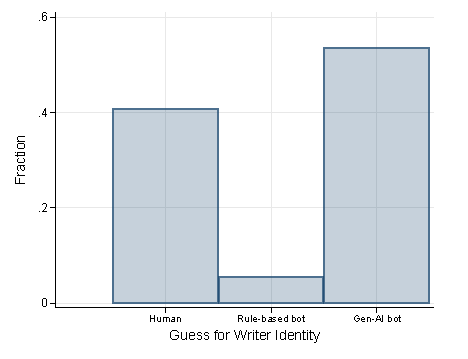
\includegraphics[width=0.6\textwidth]{GuessWriter2_Dist.pdf}
\par\end{centering}
{\small{}Notes: This figure shows the distribution of participants' guesses about the authorship of a human-written post shown in a reading task prior to the writing task. }{\small\par}
\end{figure}

The results, shown in Figure \ref{fig:read1}, indicate that readers have difficulty distinguishing between human- and AI-generated content in this setting. When the pool consists of both human- and AI-generated text, a substantial fraction of participants classify human-written posts as AI-generated. 

This finding assists interpretation of subsequent behavior in the experiment. Participants learn that human writing may plausibly be mistaken for AI-generated content (i.e., $\alpha$ is sufficiently high and $\prob(h\mid a=1)<1$). As a result, the presence of AI does not only add machine-generated messages; it also alters the informational and reputational context in which humans communicate. In particular, the possibility that human content may be perceived as AI-generated weakens the link between authored content and personal identity, a key channel in the theoretical framework.


\paragraph{Writing Task.}

In the writing task, participants are instructed to submit a short text response, with the understanding that their response may be shared in a future online survey. They are told that a future participant may read and react to their response.


The prompt reads as follows:
\begin{quote}
\textit{We have a writing task for you. For this task, we invite you to write a post on the following topic:
\\
\\
\textbf{How can you and other students in Zurich contribute to combating climate change in their daily lives?}}
\end{quote}
Participants are informed that their response will be added to a database that will be used in a follow-up survey with ETH/UZH students. In the follow-up survey, each post has a 1-in-20 chance of being randomly selected, and recipients will carefully read the selected posts and report their opinions about both the author and the post.\footnote{To isolate the effects of social image and exposure sensitivity, participants do not receive any response from the recipient. This design eliminates interaction effects and focuses attention on the sender's incentives and beliefs about how others will perceive them.}




\paragraph{Randomization. }

In a between-subjects design, participants who arrive at the writing task are cross-randomized along two dimensions: the composition of the co-senders and the identity disclosure condition.

The primary experimental manipulation is the composition of the message pool: participants are randomized with equal probability into either a condition where their message will be pooled exclusively with human-written messages or a condition where it will be pooled with a mix of human and AI-generated content. This design allows us to examine whether the presence of AI alters how people choose to communicate and express their opinions.

In the No-AI condition, participants see the following:
\begin{quote}
\textit{Your response will be added to a database of student-written posts. We will use this database in a follow-up survey with ETH/UZH students, where each post has a 1 in 20 chance of being randomly selected. In this follow-up survey, recipients will carefully read your post and share their opinion about both you and your post. They will be informed that the post is drawn from a database of 
student-written posts.}
\end{quote}
In the AI condition, participants see the same message, with the two instances of ``student-written posts'' replaced by ``75\% AI-generated posts and 25\% student-written posts.''\footnote{To ensure that AI-generated posts cannot be easily distinguished from human-generated posts on the basis of presentation, participants are informed that, if an AI-generated post is selected, it will be displayed alongside the credentials of a member of the research team.}


Participants are independently randomized into one of two identity disclosure conditions. In the identified condition, participants are informed that, upon completing the writing task, their first name (and Instagram handle, if provided), university, major, and year of study will be displayed alongside their response in the follow-up survey. In the anonymous condition, participants are informed that their response will be shared with information about their university, major, and year of study, but without any identifying information.\footnote{We implemented this follow-up as a small internal study with research team members at ETH Zurich.}  


The main difference between the identified and anonymous conditions is the disclosure of personal identifiers. For participants who did not provide an Instagram handle, only their first name is disclosed in the identified condition; for those who did, both their first name and handle are disclosed. These additional details are intended to heighten participants' concerns about exposure risks and reputational consequences -- increasing the perceived stakes of having their opinion publicly attributed to them. To maximize statistical power for testing predictions in the identified condition, participants are randomized such that 80\% are assigned to the identified condition and 20\% to the anonymous condition.

Appendix Table \ref{tab:balance} reports pre-treatment covariate balance across treatment arms. For all pairwise comparisons, F-tests of joint significance fail to reject the null hypothesis of balance, with the exception of the two anonymous arms (1)--(2), likely reflecting random variation given their small combined sample ($N = 223$). A small number of individual covariate \textit{t}-tests in other columns also fall below conventional significance levels, consistent with what would be expected given the number of comparisons.  To ensure that imbalance does not drive results in the anonymous condition, Appendix Table A3 includes pre-treatment variables (e.g., university affiliation) as controls; the coefficients on AI treatment and its interaction with identification are stable across specifications with and without these covariates.




\paragraph*{Quality control. }
Beyond including an attention check, we implement several measures to encourage effort in the writing task. Participants are instructed to complete the task in one sitting and without changing browser tabs. 
If participants switch to another browser tab during the writing task, they receive a pop-up reminder instructing them not to do so. In addition, we disable copy-and-paste functionality to reduce the likelihood that participants rely on external tools, such as ChatGPT, in the writing task. 

\subsection{Outcomes and Estimation}
Our primary outcome is whether a participant, after observing the intervention, goes on to complete the writing task and the rest of the survey.\footnote{This binarized outcome variable deviates from our pre-analysis plan. While we did pre-register the amount of effort on the task as an outcome, we did not expect participants to attrit from the study and give up their payment. See Appendix \ref{sec:pap} for details and discussion.} Given the very low attrition elsewhere in the survey, this behavioral outcome captures a binary measure of participation in content production and opinion sharing. Because participants complete an extensive baseline questionnaire before reaching the writing task, and attrition is typically low in laboratory-style samples such as ours, non-completion reflects a meaningful decision to forgo a CHF 10 (about \$12.50 USD) participation payment as well as potential lottery payments.

In addition to survey completion, we present results on several alternative measures of participation -- the length of the written response, the time spent on writing the post, and whether the response constitutes meaningful engagement with the prompt (annotated by LLM).\footnote{Responses are classified by GPT-4o-mini using a deliberately lenient threshold: a response receives a score of 1 if it is coherent and clearly related to climate change, the environment, or its consequences, and a score of 0 only if it is empty, unintelligible, or clearly unrelated to the topic (e.g., random text or spam). This criterion is designed to distinguish genuine attempts at the task from non-engagement rather than to measure response quality.} Together, these secondary measures capture variation in effort and intensity in content production and opinion sharing.

To estimate treatment effects, define $Y_{i}$ as an outcome for participant $i$ (e.g., survey completion). We compare raw means across treatment arms and assess statistical significance using two-sample t-tests. Specifically, we estimate three comparisons: (i) the difference between the anonymous and identified conditions, pooling across AI treatment status; (ii) the effect of AI presence within the anonymous condition; and (iii) the effect of AI presence within the identified condition. 

As a robustness check, we also estimate OLS specifications of the same comparisons, with and without pre-treatment covariates. Define $T_{i}$ as an indicator for whether participant $i$ was assigned to the AI treatment condition, in which their message is pooled with AI-generated content. Define $D_{i}$ as an indicator for assignment to the identified condition (Instagram handle and name may be disclosed to others). Define $\boldsymbol{X}_{i}$ as a vector of pre-treatment covariates (e.g., demographics, charitable donation decision). Our estimating equation is 
\begin{equation}
Y_{i}=\alpha+\beta T_{i}+\delta D_{i}+\theta\left(T_{i}\times D_{i}\right)
+\boldsymbol{X}_{i}'\boldsymbol{\gamma}+\varepsilon_{i}\label{eq:ATE}
\end{equation}
where $\varepsilon_{i}$ is an error term. The coefficients of interest are $\beta$, $\delta$, and $\theta$.

To study heterogeneous treatment effects, we estimate treatment effects separately across pre-specified moderators. Motivated by the model, our main heterogeneity analysis is by whether the participant shared their Instagram handle, serving as a proxy for concerns about exposure risk -- those who are willing to share their Instagram handle are less concerned about exposure risk. Further, we report heterogeneity by demographic characteristics such as age, gender, and country of origin.


\subsection{Results\label{sec:Results}}


\begin{figure}%[H]
\caption{Main Outcomes by Treatment Group \label{fig:main-results}}

\centering A. Finished Study

\begin{centering}
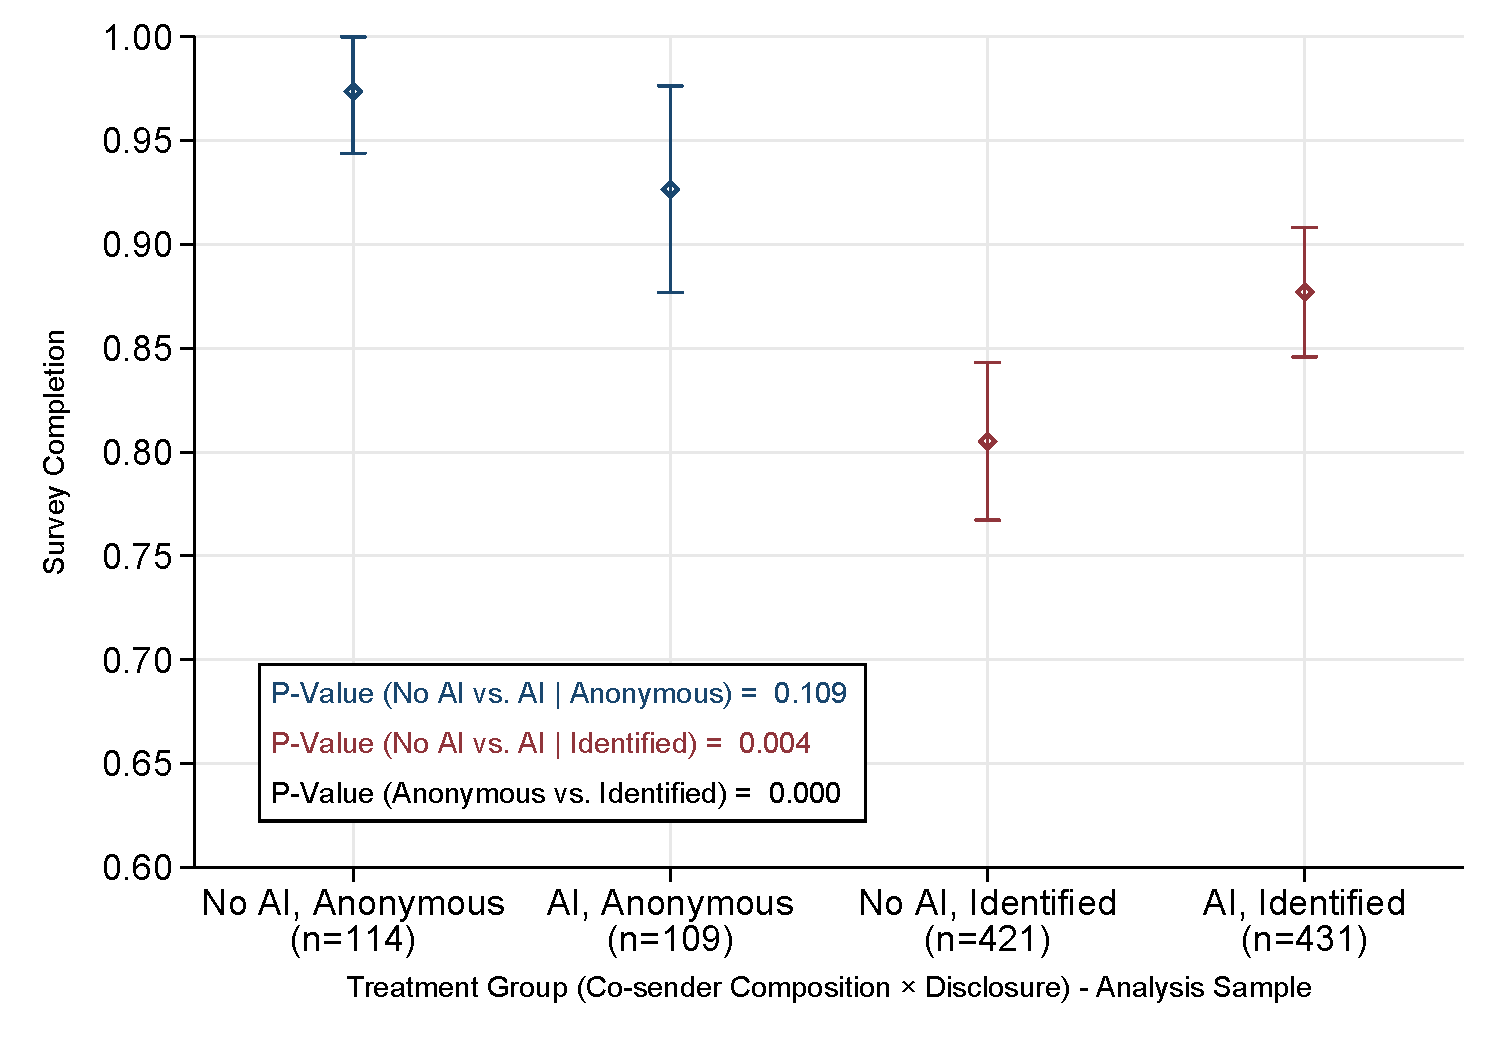
\includegraphics[width=0.7\textwidth]{ciplot_Finished_Full_raw.pdf}

\par

\end{centering}

\medskip{}


\centering B. Wrote Meaningful Post

\begin{centering}

\includegraphics[width=0.7\textwidth]{ciplot_Post_meaningfulness_Full_raw.pdf}
\par\end{centering}
\raggedright
{\small{}Notes: This figure shows our main outcomes, finishing the study (Panel A) and writing a meaningful post (Panel B), by the treatment groups. Estimates are based on the full sample of respondents who passed the attention check. Error bars indicate 95\% confidence intervals, which are truncated at 100\%.}{\small\par}
\end{figure}

\paragraph{Writing Task and Main Outcomes.}
Figure \ref{fig:main-results} reports the main results for the writing task. Each plot shows the outcome means by treatment group with 95\% confidence intervals. We report two main outcomes: Panel A shows completion of the study, while Panel B shows whether participants wrote a meaningful post.\footnote{Appendix Figure \ref{fig:post-length} shows similar results for the number of characters written.} The four treatment groups, from left to right, are (a) only human co-senders (no AI) and not identified (anonymous), (b) 75\% AI co-senders (AI) and not identified, (c) human co-senders and identified (by first name, and if applicable, Instagram handle), and (d) AI co-senders and identified. 

Consider first the anonymous condition, represented by the first two estimates in blue in Figure~\ref{fig:main-results}.  Completion rates are high and similar across AI conditions. In Panel A, completion is approximately 97 percent in the no-AI condition (first group) and 93 percent in the AI condition (second group), and the difference is not statistically significant ($p\text{ value} = 0.109$). A similar pattern holds for writing a meaningful post in Panel B, where participation remains high and the difference between AI and no-AI conditions is small and statistically insignificant ($p\text{ value} = 0.321$). This is consistent with the model's prediction that, in the absence of exposure risks, AI would not increase participation and may slightly reduce it by weakening signaling incentives.

Now consider the estimates in red, where participants are identified. Here, in contrast, outcomes decrease sharply relative to the anonymous condition. In the no-AI condition, identification substantially reduces participation (third group, relative to first group). Completion (Panel A) falls to roughly 80 percent, and the share writing a meaningful post (Panel B) drops to about 78 percent. These declines are large relative to the anonymous conditions and are highly statistically significant ($p\text{ value} < 0.001$). This pattern aligns with Proposition \ref{prop:comparative_statics} Part (i), which predicts that identity disclosure increases exposure risk and discourages participation.


Next, comparing the third group to the fourth group, we see that the presence of AI mitigates identification effects on participation. When AI co-senders are present, completion rises from about 80 percent to nearly 88 percent ($p\text{ value} = 0.004$), and the probability of writing a meaningful post increases from about 78 percent to 86 percent ($p\text{ value} = 0.003$). These gains are sizable and statistically significant, and they reverse a substantial portion of the participation loss induced by identification. This is consistent with predictions of the model in Proposition \ref{prop:comparative_statics} Part (iii), in which AI reduces exposure risk by weakening the perceived link between authored content and personal identity.\footnote{Proposition \ref{prop:comparative_statics} Part (ii) predicts that stronger image concern increases participation. We do try to measure image concerns at baseline, but we do not experimentally manipulate it. Thus we cannot directly test this prediction. That is an interesting area for future work.}

Appendix Table \ref{tab:treat_effect} presents these results in regression form, without controls, with demographic controls, and with the full set of pre-treatment controls. We find the same result with stable coefficients across specifications: identification reduces survey completion, and AI presence mitigates this effect.


It is worth emphasizing that completion of the study is a high-stakes outcome. Participants reached the writing task only after completing a lengthy baseline survey, so attrition at this stage reflects a costly decision to disengage and leave a significant payment (10 CHF) on the table. Attrition is typically low in surveys of this type, a fact reflected in the very high completion rates in the anonymous conditions. The sharp drop in completion under identification, and its partial reversal with AI presence, therefore indicates meaningful changes in participation incentives rather than noise or fatigue.

We treat survey completion as the primary outcome and interpret post-task measures with caution, as they are subject to selection from differential attrition. For example, willingness to pay to remove the post is observed only for participants who completed the writing task. Because participants who drop out under the Identified condition are plausibly those most sensitive to exposure risk, the completer sample is selected toward individuals with lower exposure concerns. This truncation attenuates treatment differences in post-task outcomes and may explain why willingness to pay to remove the post does not differ significantly across AI conditions (Appendix Figure \ref{fig:wtp}).


\begin{figure}[t]%[H]
\caption{Heterogeneous Effects by Exposure Sensitivity \label{fig:privacy}}

\medskip{}

\begin{centering}
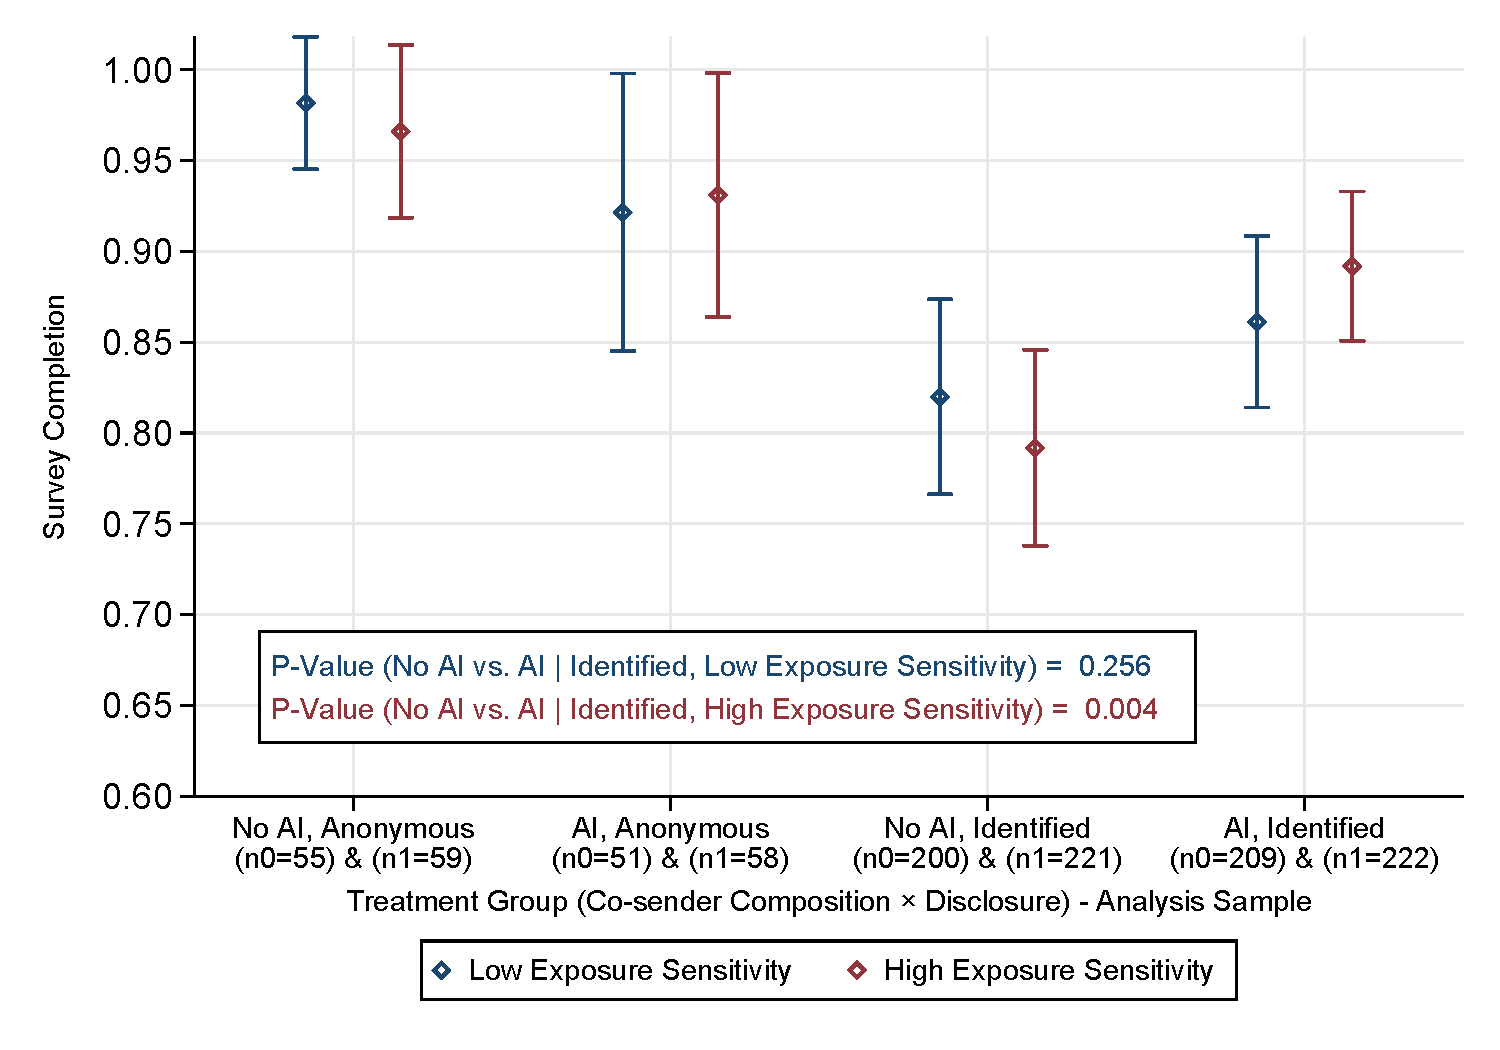
\includegraphics[width=0.8\textwidth]{ciplot_Finished_hte_not_shared_handle_Full_raw.pdf}
\par\end{centering}
{\small{}Notes: This figure reports treatment effects on study completion by exposure-risk concern, proxied by willingness to share Instagram handle. Estimates are based on respondents who passed the attention check. Error bars denote 95\% confidence intervals.}{\small\par}
\end{figure}

\paragraph{Heterogeneity by Baseline Exposure Sensitivity.} Motivated by the model, we explore heterogeneity by sensitivity to exposure risk. Specifically, a participant's level of exposure risk concern is measured by their willingness to share their personal Instagram handle. Participants who chose to share their handle are classified as having low exposure sensitivity, while those who did not are classified as having high exposure sensitivity.  Figure \ref{fig:privacy} plots variation in the ``finished study'' outcome by treatment group (corresponding to Figure \ref{fig:main-results} Panel A), with the outcome means further split by sensitivity to exposure risk.\footnote{In Figure \ref{fig:privacy}, high exposure sensitivity group includes both non-users and Instagram users who choose not to share their handle. Appendix Figure \ref{fig:privacy-instagram} shows that these heterogeneity results hold when limiting to the sample of participants who uses Instagram.}


First, comparing the first two groups, exposure sensitivity does not affect participation under anonymity. Consistent with the model, exposure risks are not triggered under anonymity so neither AI nor exposure sensitivity should matter.

Turning to the identified treatments, the third and fourth groups, there is clear heterogeneity. Comparing the first (No AI, Anonymous) and third (No AI, Identified) groups, the negative effect of being identified on participation is substantially larger for participants with high exposure sensitivity (in red) than those with low exposure sensitivity (in blue). Under the third group (No AI, Identified), completion rates are markedly lower for those with high exposure sensitivity. Consistent with the model, participants who are more sensitive to exposure face higher perceived costs from having their content linked to their identity, and therefore are more likely to disengage when there is risk of exposure. 


Finally, comparing the third group (no AI, identified) to the fourth group (AI, identified), the mitigating effect of AI presence is stronger among participants with higher exposure sensitivity. When AI co-senders are present, completion rates increase more for individuals with higher sensitivity (in red) than for those with lower sensitivity (in blue). This result suggests that AI is especially effective at reducing perceptions of exposure risk for individuals who are most sensitive to them. In the language of the model, AI more strongly weakens the perceived mapping between authored content and personal identity for these participants, thereby restoring participation incentives.


These heterogeneity patterns reinforce the proposed mechanism. The main effects are not driven by generic reactions to AI or survey fatigue, but by differential exposure sensitivity across participants. Notably, the high-sensitivity group faces objectively less disclosure: in the identified condition, participants with low exposure sensitivity have both their name and Instagram handle disclosed, while those with high exposure sensitivity have only their first name disclosed.  The fact that the interaction between disclosure and AI presence is largest among those with greater sensitivity to exposure risk -- who, if anything, face less objective disclosure -- provides direct evidence that AI operates through the exposure risk channel highlighted in the theoretical framework. The same qualitative patterns appear both in the full sample and in the Instagram-user subsample, indicating that the results are not driven by platform usage or selective participation.



\paragraph{Heterogeneity by Demographics.}

Appendix \ref{sec:app_results} includes heterogeneity results along additional demographic dimensions. Younger participants are more likely to drop out than older participants across all treatment conditions (Appendix Figure \ref{fig:age}), but treatment and interaction effects are similar. Swiss participants are more responsive to identification than non-Swiss participants (Appendix Figure \ref{fig:nationality}), but there is no heterogeneity in the response to AI.  

We do find heterogeneity by gender, however (Appendix Figure \ref{fig:gender}). Women report higher exposure sensitivity than men, and the treatment effects differ accordingly. Under identification, women are more likely to disengage in the absence of AI. The presence of AI under identification leads to a larger increase in participation for women than for men. 


\section{Conclusion}

Many online platforms are built around social interaction and identity, yet these environments increasingly include artificial agents that are difficult to distinguish from humans. This paper develops a signaling framework in which participation in content production yields social image benefits but may also impose exposure costs when authorship can be linked to identity. We show that the presence of generative AI alters human participation by weakening the perceived connection between content and personal identity. In an online writing experiment, making participants identifiable sharply reduces participation, even late in a paid survey. However, introducing AI co-senders substantially mitigates this effect. When participants remain anonymous, AI has little or no positive effect on participation. These patterns are strongest among participants with higher exposure sensitivity and among women. Together, the results show that AI reshapes human content production not only by generating text, but by changing the incentives faced by human contributors, complementing evidence that AI tools also reshape productivity and behavior in knowledge work \citep{noy2023experimental,brynjolfsson2024generative,mehmood2026courts}.

Our findings clarify why the effects of AI on human engagement can appear contradictory across settings. When participation primarily serves as a signal of prosocial motivation, the presence of AI dilutes signaling value and can discourage human contributions. By contrast, when participation carries meaningful risk of exposing sensitive views, AI can increase engagement by attenuating perceived exposure. This distinction helps reconcile concerns that AI may crowd out human expression with evidence that AI can sometimes expand participation, consistent with recent work showing that generative AI can both dilute communication signals and reshape incentives for communication \citep{cowgill2024cheapen,cui2025signaling,galdin2025making}. Whether AI reduces or increases human engagement depends on how strongly content is tied to personal identity and how costly that linkage is perceived to be.

The results also speak directly to platform design. Decisions about attribution, identity disclosure, and the visibility of AI-generated content are not neutral and not independent. By shaping the extent to which authored content is perceived as uniquely human, platforms influence who chooses to speak and who remains silent. In environments where exposure risks are salient, introducing AI or reducing certainty about authorship may broaden participation, particularly among users who are more sensitive to exposure risk. Conversely, in settings where reputation and signaling are central, the same design choices may weaken incentives to contribute. These choices interact with platform incentives to promote engagement, which can shape the informational environment users face \citep{siderius2023,cookson2024}.

Several avenues for future research follow naturally. First, repeated interaction and feedback may amplify or dampen the exposure-risk mechanism we identify, especially as users update beliefs about AI prevalence and attribution over time. Second, richer attribution regimes, such as probabilistic labeling or optional identity disclosure, could allow users to sort into environments that better match their preferences. Finally, understanding how AI affects participation in higher-stakes domains such as political speech, workplace communication, or mental health forums remains a high-value area, with initial results suggesting that humans behave differently when interacting with machines rather than humans \citep{marechal2020,chugunova2022we,bogliacino2023}. More broadly, our results suggest that as AI becomes embedded in social environments, its most consequential effects may arise not from what machines say, but from how their presence reshapes the social meaning of human speech.


\newpage\leftskip=0em 
\parindent=-2em
\onehalfspacing

\bibliographystyle{aea}
\bibliography{references}

\parindent=2em
\leftskip=0em

\clearpage{}

\pagebreak{}

\appendix

\setcounter{figure}{0} \renewcommand{\thefigure}{A\arabic{figure}}

\setcounter{table}{0} \renewcommand{\thetable}{A\arabic{table}}\pagestyle{fancy}


\noindent {{\LARGE \textbf{Appendix} }}
\section{Model Appendix}\label{appendix:theoretical framework}

Define the operator $\Phi(v)\triangleq v - c + \pi(v)T(v)$, where $\pi(v)T(v)$ captures the indirect payoff from participation through prosocial image and exposure channels. We say that participation decisions exhibit \textit{strategic complementarity} if $(\pi(v)T(v))'<0$ and \textit{strategic substitutes} if $(\pi(v)T(v))'>0$. To see the intuition, note that a marginal expansion of participation corresponds to a decrease in the cutoff $v$. Lowering the cutoff has two opposing effects on the indirect payoff from participation: it raises the probability that a participant is human, but also lowers the expected intrinsic motivation. As a result, the overall effect on the indirect payoff $\pi(v)T(v)$ is ambiguous. When $(\pi(v)T(v))'<0$, the increase in perceived human identity dominates the decline in expected type, so a marginal expansion of participation raises the indirect payoff from participation, generating strategic complementarity. Conversely, when $(\pi(v)T(v))'>0$, the decline in expected type dominates, so a marginal expansion lowers the indirect payoff and participation decisions are strategically substitutable.


The sign and magnitude of $(\pi(v)T(v))'$ further determine equilibrium stability. Since $\Phi'(v) = 1+(\pi(v)T(v))'$, the response of marginal types to a small expansion of participation depends on whether the induced change in the indirect payoff is strong enough to offset the decline in intrinsic motivation at the margin. When $(\pi(v)T(v))'<-1$, the increase in the indirect payoff dominates the loss in intrinsic motivation, so marginal types in $[v^*-\diff v,v^*]$, who initially preferred to abstain, now strictly prefer to participate. This self-reinforcing feedback leads to further participation and continued improvement of the participation pool, implying that only corner equilibria are locally stable. By contrast, when $(\pi(v)T(v))'>-1$, either complementarity is too weak or participation decisions are strategically substitutable, the improvement in the indirect payoff is insufficient to overturn the marginal loss in intrinsic motivation. As a result, types just below the cutoff continue to prefer abstention following a small expansion of participation, and the interior cutoff equilibrium is locally stable.

To ensure a unique stable equilibrium, we impose $\Phi'(v)>0$ on $(\underline v,\overline v)$ in Proposition \ref{prop:equilibrium}. This condition is always satisfied when participation decisions are strategic substitutes, or when they are strategic complements but the complementarity is sufficiently weak so that the induced increase in the indirect payoff does not outweigh the marginal decline in intrinsic motivation.

\begin{proof}[Proof of Proposition \ref{prop:equilibrium}]
    Consider a candidate cutoff $v^*$. The marginal type $v^*$ is indifferent between participation and abstention if and only if $u_0 = \Phi(v^*)$. Under the assumption that $\Phi'(v)>0$ on $(\underline v,\overline v)$, the equation $\Phi(v)=u_0$ has at most one solution. If $u_0\in(\Phi(\underline v),\Phi(\overline v))$, existence of a solution $v^*\in(\underline v,\overline v)$ follows from continuity and the intermediate value theorem, and uniqueness follows from strict monotonicity, establishing (i). If $u_0\ge \Phi(\overline v)$, then $\Phi(v)\le u_0$ for all $v$, so no type strictly prefers participation; thus $a=0$ for all $v$, establishing (ii). The argument for (iii) is symmetric.
\end{proof}


\begin{proof}[Proofs of Proposition \ref{prop:comparative_statics}]
    For an interior equilibrium, $v^*$ solves the indifference condition
    \[
    u_0=\Phi(v^*)=v^*-c+\pi(v^*)T(v^*).
    \]
    Since $\Phi'(v^*)>0$, the implicit function theorem applies and yields, for any parameter $\theta$,
    \[
    \frac{\partial v^*}{\partial \theta}=-\frac{\partial_\theta\Phi(v^*)}{\Phi'(v^*)},
    \]
    so the sign of $\partial v^*/\partial\theta$ is the opposite of the sign of $\partial_\theta\Phi(v^*)$.


    \emph{(i) $\theta=\gamma$.} The parameter $\gamma$ enters $\Phi$ only through $T(v^*)=\mu\,E[v\mid v\ge v^*]-\gamma$. Thus
    \[
    \partial_\gamma\Phi(v^*)=\pi(v^*)\,\partial_\gamma T(v^*)=-\pi(v^*)<0,
    \]
    so $\partial v^*/\partial\gamma>0$.
    
    \emph{(ii) $\theta=\mu$.} The parameter $\mu$ enters $\Phi$ only through $T(v^*)=\mu\,E[v\mid v\ge v^*]-\gamma$. Thus
    \[
    \partial_\mu\Phi(v^*)=\pi(v^*)\,\partial_\mu T(v^*)=\pi(v^*)\,E[v\mid v\ge v^*]>0,
    \]
    so $\partial v^*/\partial\mu<0$.
    

    \emph{(iii) $\theta = \rho,\alpha$.} The parameters $\rho$ and $\alpha$ enter $\Phi$ only through $\pi(\cdot)$. Hence
    \[
    \partial_\rho\Phi(v^*)=T(v^*)\,\partial_\rho\pi(v^*),\qquad
    \partial_\alpha\Phi(v^*)=T(v^*)\,\partial_\alpha\pi(v^*).
    \]
    From the expression $\pi(v) = \frac{(1-\rho)(1-F(v))}{\rho \alpha + (1-\rho)(1-F(v))}$, we have $\partial_\rho\pi(v^*)<0$ and $\partial_\alpha\pi(v^*)<0$ (a higher Gen-AI bot share or a higher mimicry rate lowers the posterior probability that a participant is human). It follows that $\partial_\rho\Phi(v^*)$ and $\partial_\alpha\Phi(v^*)$ have the opposite sign of $T(v^*)$, implying that $\partial v^*/\partial\rho$ and $\partial v^*/\partial \alpha$ have the same sign as $T(v^*)$. This establishes (iii).
\end{proof}


\clearpage

\section{Experiment Appendix\label{app:Design}}

\subsection{Appendix Results \label{sec:app_results}}


\begin{table}[H]
\caption{Sample Demographics}
\label{tab:summary_stat}
\centering
\scalebox{0.9}{\input{summary_stat}}


\vspace{0.5em}
\begin{minipage}{0.9\textwidth}
\footnotesize
\raggedright
\textit{Notes:} Column 1 presents average demographics for the full eligible sample in this study. 
Column 2 presents average demographics of all residents of Switzerland aged 18 or older using 
data from the 2023 Swiss Federal Statistical Office (FSO) Population and Households Statistics 
(STATPOP), the FSO Structural Survey and Swiss Labour Force Survey (for educational attainment 
and migration status), and official 2023 National Council election statistics.
\end{minipage}


\end{table}

\begin{table}[htbp]
    \caption{Summary Statistics and Balance Tests}
    \label{tab:balance}
    \centering
    \resizebox{\textwidth}{!}{\begin{tabular}{l*{8}{c}}
\hline\hline
& \multicolumn{4}{c}{Summary Statistics}
& \multicolumn{4}{c}{\textit{p}-values} \\
& (1) & (2) & (3) & (4)
& (1)--(2) & (3)--(4) & (1)--(3) & (1,2)--(3,4) \\
& No AI, Anon. & AI, Anon. & No AI, Ident. & AI, Ident.
& & & & \\
& Mean/SD & Mean/SD & Mean/SD & Mean/SD & & & & \\
\hline
Age             &   23.868&   24.312&   23.534&   23.742&    0.459&    0.305&    0.378&    0.156\\
                &  (3.745)&  (5.055)&  (2.853)&  (3.061)&         &         &         &         \\
Gender (Female) &    0.509&    0.523&    0.487&    0.543&    0.833&    0.102&    0.681&    0.991\\
                &  (0.502)&  (0.502)&  (0.500)&  (0.499)&         &         &         &         \\
Swiss           &    0.491&    0.486&    0.508&    0.452&    0.941&    0.103&    0.747&    0.817\\
                &  (0.502)&  (0.502)&  (0.501)&  (0.498)&         &         &         &         \\
Graduate Student&    0.509&    0.450&    0.534&    0.557&    0.378&    0.512&    0.628&    0.080\\
                &  (0.502)&  (0.500)&  (0.499)&  (0.497)&         &         &         &         \\
Voted in Last Election&    0.430&    0.376&    0.501&    0.427&    0.416&    0.030&    0.176&    0.107\\
                &  (0.497)&  (0.487)&  (0.501)&  (0.495)&         &         &         &         \\
ETH             &    0.763&    0.596&    0.724&    0.654&    0.008&    0.027&    0.397&    0.834\\
                &  (0.427)&  (0.493)&  (0.447)&  (0.476)&         &         &         &         \\
Donation (CHF)  &   22.500&   19.349&   23.183&   24.659&    0.350&    0.449&    0.809&    0.128\\
                & (26.325)& (23.926)& (28.407)& (28.495)&         &         &         &         \\
Instagram User  &    0.816&    0.761&    0.793&    0.814&    0.323&    0.440&    0.589&    0.630\\
                &  (0.389)&  (0.428)&  (0.405)&  (0.389)&         &         &         &         \\
Image Concern (1-5)&    2.298&    2.385&    2.446&    2.367&    0.514&    0.278&    0.156&    0.390\\
                &  (0.968)&  (1.018)&  (1.022)&  (1.077)&         &         &         &         \\
Exposure Sensitivity&    0.518&    0.532&    0.525&    0.515&    0.829&    0.774&    0.889&    0.900\\
                &  (0.502)&  (0.501)&  (0.500)&  (0.500)&         &         &         &         \\
Climate Concern Index&    0.018&   -0.000&   -0.015&    0.010&    0.874&    0.677&    0.712&    0.858\\
                &  (0.841)&  (0.888)&  (0.861)&  (0.861)&         &         &         &         \\
AI Familiarity (1-5)&    4.544&    4.505&    4.518&    4.459&    0.678&    0.231&    0.709&    0.493\\
                &  (0.654)&  (0.753)&  (0.678)&  (0.742)&         &         &         &         \\
AI Persuasion (1-5)&    3.237&    3.569&    3.397&    3.434&    0.014&    0.560&    0.148&    0.828\\
                &  (1.067)&  (0.937)&  (0.940)&  (0.922)&         &         &         &         \\
Base-Task Perceived Difference from AI (1-5)&    3.649&    3.716&    3.679&    3.759&    0.587&    0.210&    0.756&    0.582\\
                &  (0.931)&  (0.893)&  (0.878)&  (0.966)&         &         &         &         \\
React to Example Post&    0.246&    0.202&    0.211&    0.232&    0.435&    0.469&    0.449&    0.940\\
                &  (0.432)&  (0.403)&  (0.409)&  (0.423)&         &         &         &         \\
React to Post 1 in Reading Task&    0.456&    0.376&    0.352&    0.420&    0.227&    0.040&    0.047&    0.405\\
                &  (0.500)&  (0.487)&  (0.478)&  (0.494)&         &         &         &         \\
React to Post 2 in Reading Task&    0.342&    0.239&    0.316&    0.350&    0.089&    0.287&    0.602&    0.226\\
                &  (0.477)&  (0.428)&  (0.465)&  (0.478)&         &         &         &         \\
Guess Human Writer for Post 1&    0.667&    0.798&    0.708&    0.747&    0.026&    0.199&    0.408&    0.923\\
                &  (0.473)&  (0.403)&  (0.455)&  (0.435)&         &         &         &         \\
Guess Human Writer for Post 2&    0.342&    0.358&    0.406&    0.439&    0.807&    0.340&    0.208&    0.045\\
                &  (0.477)&  (0.482)&  (0.492)&  (0.497)&         &         &         &         \\
Customer Support Bot (1-5)&    2.974&    3.018&    2.974&    2.854&    0.763&    0.096&    0.999&    0.316\\
                &  (1.026)&  (1.178)&  (1.034)&  (1.067)&         &         &         &         \\
Social Media Bot (1-5)&    1.798&    1.697&    1.696&    1.696&    0.439&    0.999&    0.326&    0.470\\
                &  (0.988)&  (0.957)&  (0.970)&  (0.973)&         &         &         &         \\
\textit{N} & 114 & 109 & 421 & 431
& 223 & 852 & 535 & 1075 \\
\midrule
F-test of joint significance (F-statistic)
& & & &
& 2.13 & 1.43 & 0.96 & 1.48 \\
F-test, number of observations
& & & &
& 223 & 845 & 529 & 1068 \\
\hline\hline
\end{tabular}}
    \begin{minipage}{\textwidth}
        \footnotesize\medskip
        \textit{Notes:} Columns 1--4 report means with standard deviations
        in parentheses by treatment arm: (1) No AI \& Anonymous,
        (2) AI \& Anonymous, (3) No AI \& Identified, (4) AI \& Identified.
        Columns 5--8 report \textit{p}-values from unequal-variance
        \textit{t}-tests for each pairwise comparison. The bottom rows
        report the F-statistic and number of observations from a joint
        significance test of all covariates predicting treatment assignment.
    \end{minipage}
\end{table}




\begin{table}[htbp]
\caption{Treatment Effects on Finishing Study}
\label{tab:treat_effect}
\centering

\scalebox{0.58}{\begin{tabular*}{\hsize}{@{\hskip\tabcolsep\extracolsep\fill}l*{3}{c}}
\toprule
                &\multicolumn{1}{c}{(1)}&\multicolumn{1}{c}{(2)}&\multicolumn{1}{c}{(3)}\\
                &\multicolumn{1}{c}{No Controls}&\multicolumn{1}{c}{Demographics}&\multicolumn{1}{c}{All Controls}\\
\midrule
Identified Treatment&   -0.168***&   -0.170***&   -0.161***\\
                &  (0.024)   &  (0.025)   &  (0.025)   \\
\addlinespace
AI Treatment    &   -0.047   &   -0.048   &   -0.039   \\
                &  (0.029)   &  (0.030)   &  (0.032)   \\
\addlinespace
AI $\times$ Identified&    0.119** &    0.120** &    0.109** \\
                &  (0.038)   &  (0.039)   &  (0.040)   \\
\addlinespace
Age 25 Or Older &            &    0.051*  &    0.047*  \\
                &            &  (0.023)   &  (0.023)   \\
\addlinespace
Gender (Female) &            &   -0.100***&   -0.097***\\
                &            &  (0.022)   &  (0.022)   \\
\addlinespace
Swiss           &            &   -0.075** &   -0.068*  \\
                &            &  (0.029)   &  (0.029)   \\
\addlinespace
Graduate Student&            &    0.000   &    0.005   \\
                &            &  (0.024)   &  (0.025)   \\
\addlinespace
ETH             &            &   -0.012   &   -0.012   \\
                &            &  (0.024)   &  (0.024)   \\
\addlinespace
Voted in Last Election&            &    0.022   &    0.021   \\
                &            &  (0.028)   &  (0.028)   \\
\addlinespace
Instagram User  &            &            &   -0.045   \\
                &            &            &  (0.028)   \\
\addlinespace
Exposure Sensitivity&            &            &   -0.003   \\
                &            &            &  (0.025)   \\
\addlinespace
Image Concern Above Median&            &            &   -0.010   \\
                &            &            &  (0.021)   \\
\addlinespace
Donated         &            &            &   -0.001   \\
                &            &            &  (0.022)   \\
\addlinespace
Frequent AI User&            &            &    0.026   \\
                &            &            &  (0.023)   \\
\addlinespace
High AI Persuasion&            &            &   -0.024   \\
                &            &            &  (0.021)   \\
\addlinespace
Base-Task Perceived Distinct from AI&            &            &    0.004   \\
                &            &            &  (0.022)   \\
\addlinespace
React to Example Post&            &            &    0.059*  \\
                &            &            &  (0.024)   \\
\addlinespace
React to Post 1 in Reading Task&            &            &    0.063** \\
                &            &            &  (0.022)   \\
\addlinespace
React to Post 2 in Reading Task&            &            &   -0.016   \\
                &            &            &  (0.024)   \\
\addlinespace
Guess Human Writer for Post 1&            &            &   -0.022   \\
                &            &            &  (0.024)   \\
\addlinespace
Guess Human Writer for Post 2&            &            &    0.010   \\
                &            &            &  (0.022)   \\
\addlinespace
Prefer Customer Support Bot&            &            &    0.023   \\
                &            &            &  (0.022)   \\
\addlinespace
Prefer AI On Social Media&            &            &   -0.013   \\
                &            &            &  (0.027)   \\
\addlinespace
Constant        &    0.974***&    1.044***&    1.042***\\
                &  (0.015)   &  (0.033)   &  (0.056)   \\
\midrule
Adj. \(R^2\)    &    0.024   &    0.052   &    0.060   \\
\(N\)           &    1,075   &    1,075   &    1,075   \\
\bottomrule
\end{tabular*}}

\vspace{0.5em}
\begin{minipage}{\textwidth}
\footnotesize
\raggedright
\textit{Notes:} This table reports OLS estimates of the effect of
    treatment assignment on finishing the study.
    The omitted category is the No AI \& Anonymous arm.
    \textit{Identified Treatment} is an indicator for being assigned
    to the identified condition; \textit{AI Treatment} is an indicator
    for being assigned to the AI condition;
    \textit{AI $\times$ Identified} is their interaction.
    Column~1 includes no controls, Column~2 adds demographic controls, and Column~3 further adds
    pre-treatment behavioral and attitudinal controls. Robust standard errors in parentheses.
    $^{+} p<0.10, ^{*} p<0.05, ^{**} p<0.01, ^{***} p<0.001$.
\end{minipage}

\end{table}




\begin{figure}%[H]
\caption{Post Length and Time Spent by Treatment Group \label{fig:post-length}}
\begin{centering}
A. Post Length\\[0.5em]
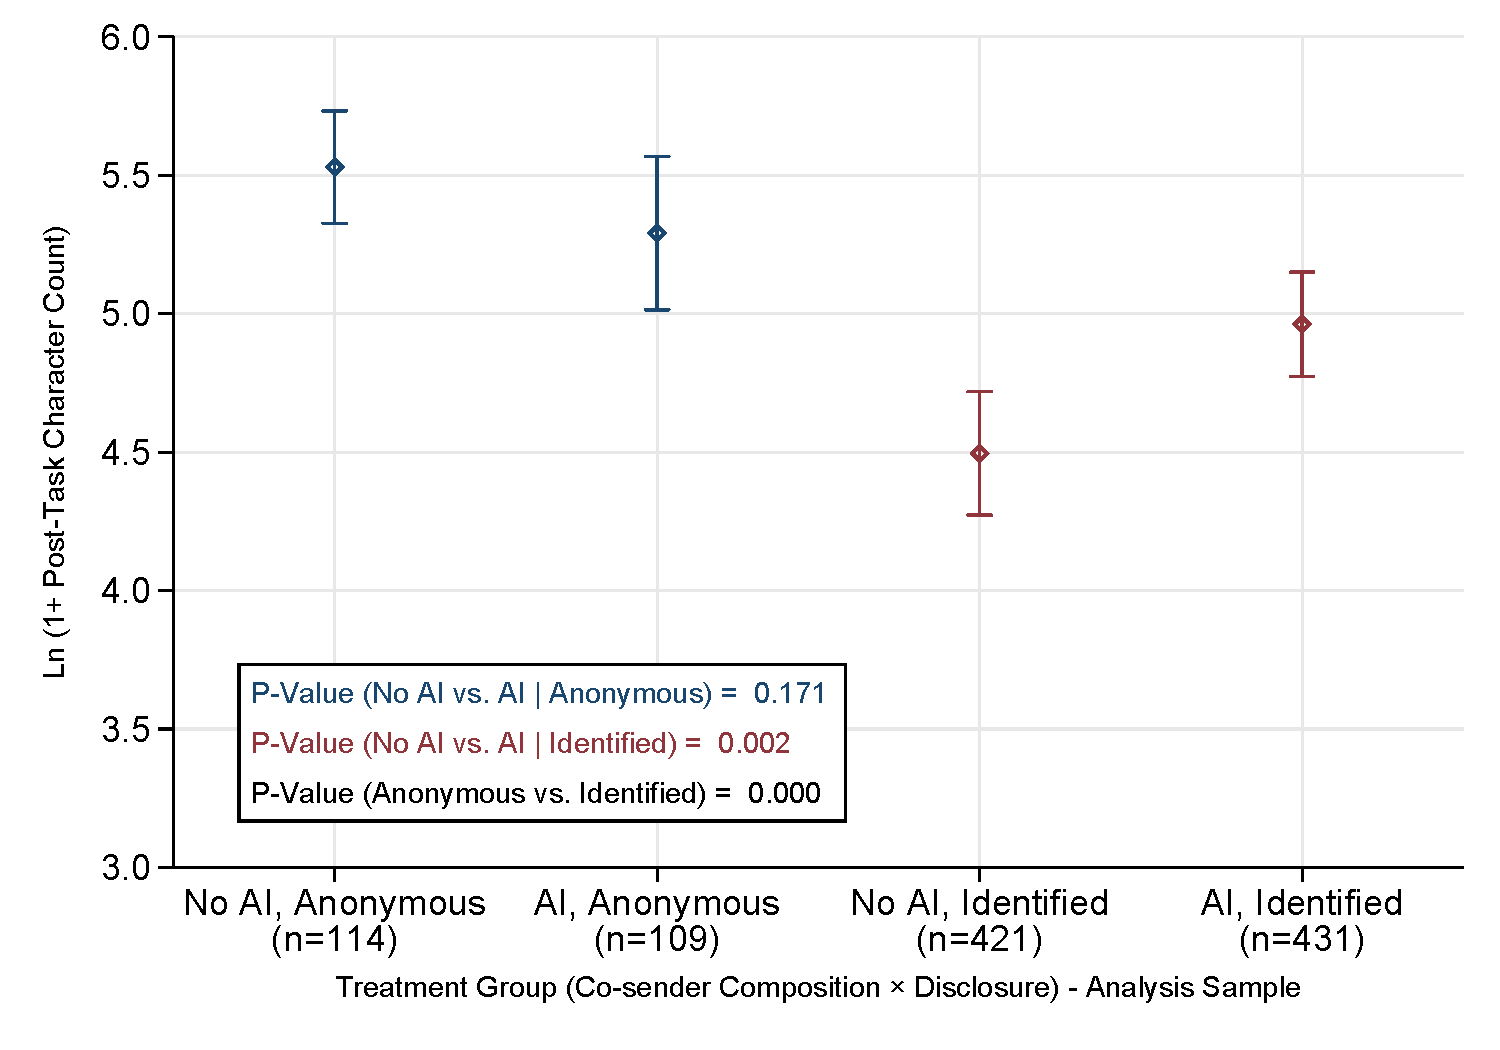
\includegraphics[width=0.7\textwidth]{ciplot_Post_TextLength_log_Full_raw.pdf}
\par
\end{centering}
\medskip{}
\begin{centering}
B. Time Spent on Post\\[0.5em]
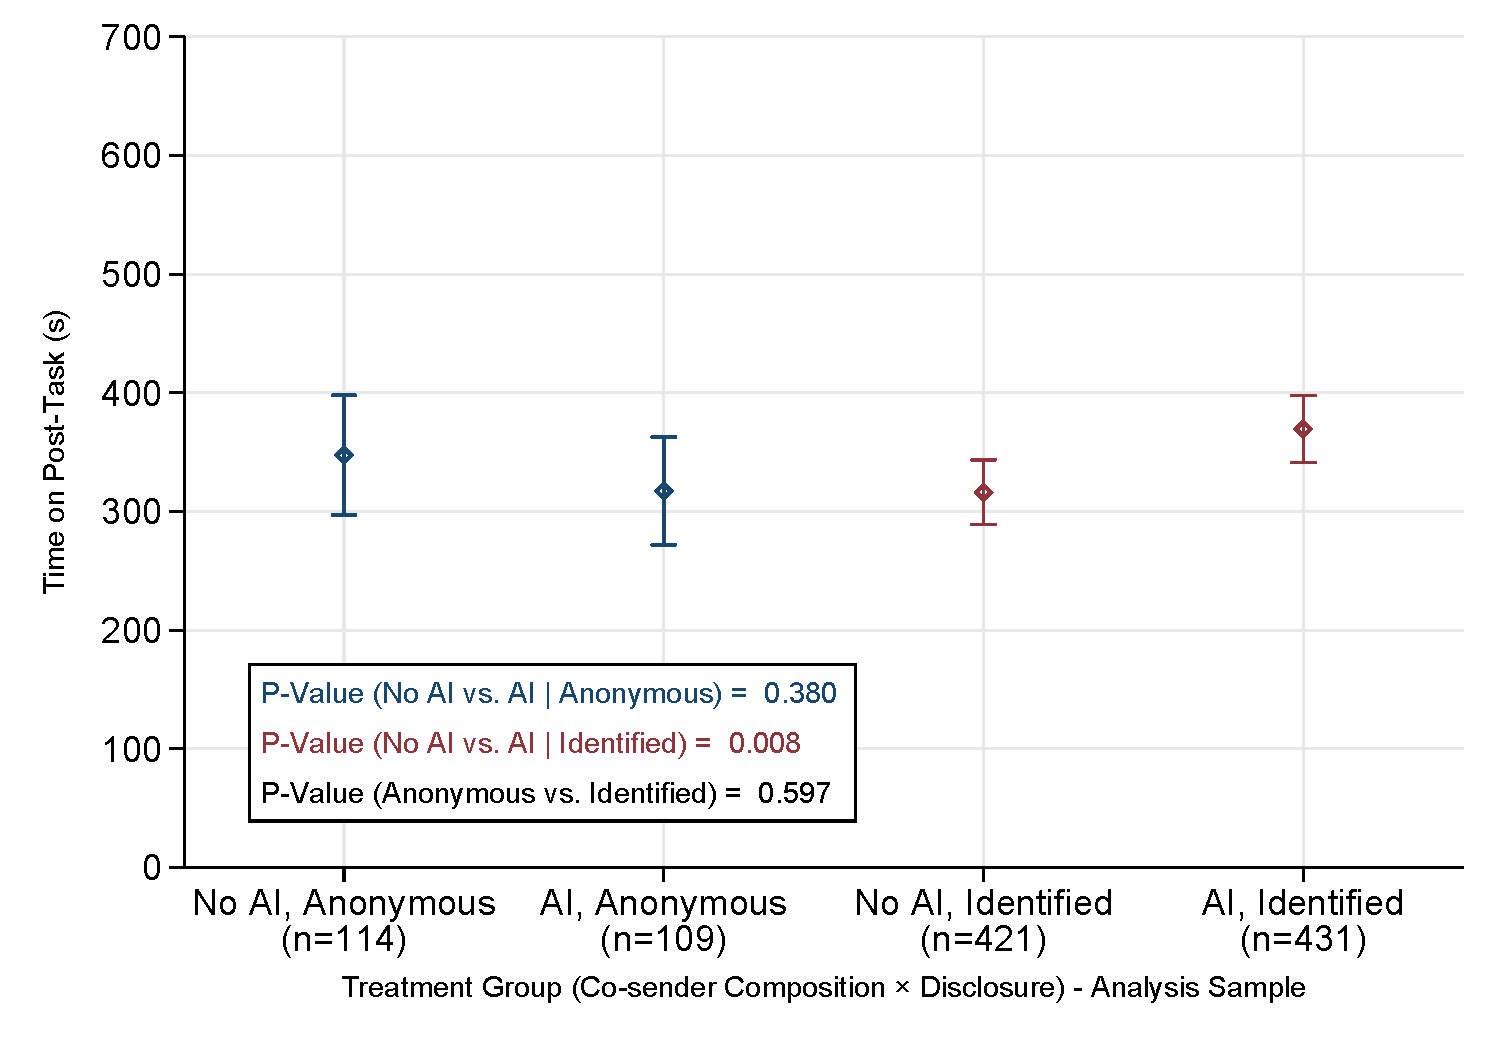
\includegraphics[width=0.7\textwidth]{ciplot_TimePost_W_Full_raw.pdf}
\par
\end{centering}
\raggedright
{\small{}Notes: This figure shows post length and time spent by treatment group. Panel A reports post length and Panel B reports time spent on the post (in seconds). For respondents who did not write a post, post length and time spent are imputed to zero. Time spent is winsorized at 95\%. Estimates are based on the full sample of respondents who passed the attention check. Error bars indicate 95\% confidence intervals.}{\small\par}
\end{figure}


\begin{figure}[H]
\caption{Heterogeneous Effects by Exposure Sensitivity --- Instagram User Sample \label{fig:privacy-instagram}}
\medskip{}
\begin{centering}
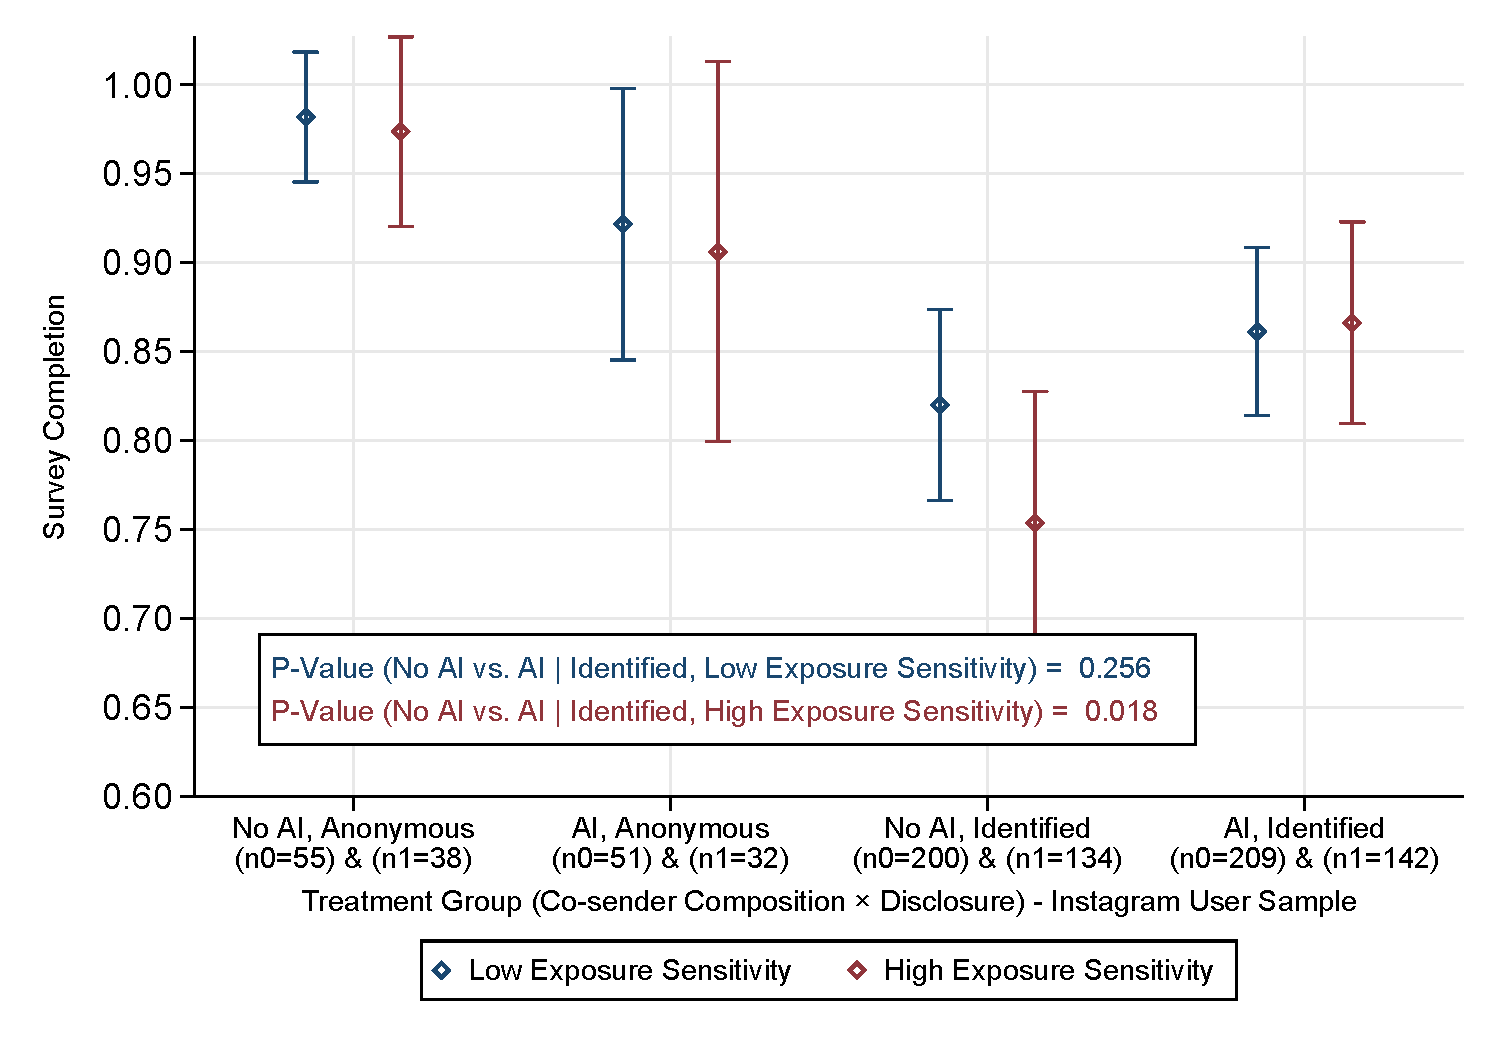
\includegraphics[width=0.8\textwidth]{ciplot_Finished_hte_not_shared_handle_IGUsers_raw.pdf}
\par\end{centering}
{\small{}Notes: This figure reports treatment effects on study completion by exposure-risk concern, proxied by willingness to share Instagram handle, for the Instagram user sample. Estimates are based on respondents who passed the attention check. Error bars denote 95\% confidence intervals.}{\small\par}
\end{figure}


\begin{figure}[H]
\caption{Heterogeneity by Age \label{fig:age}}

\medskip{}

\begin{centering}
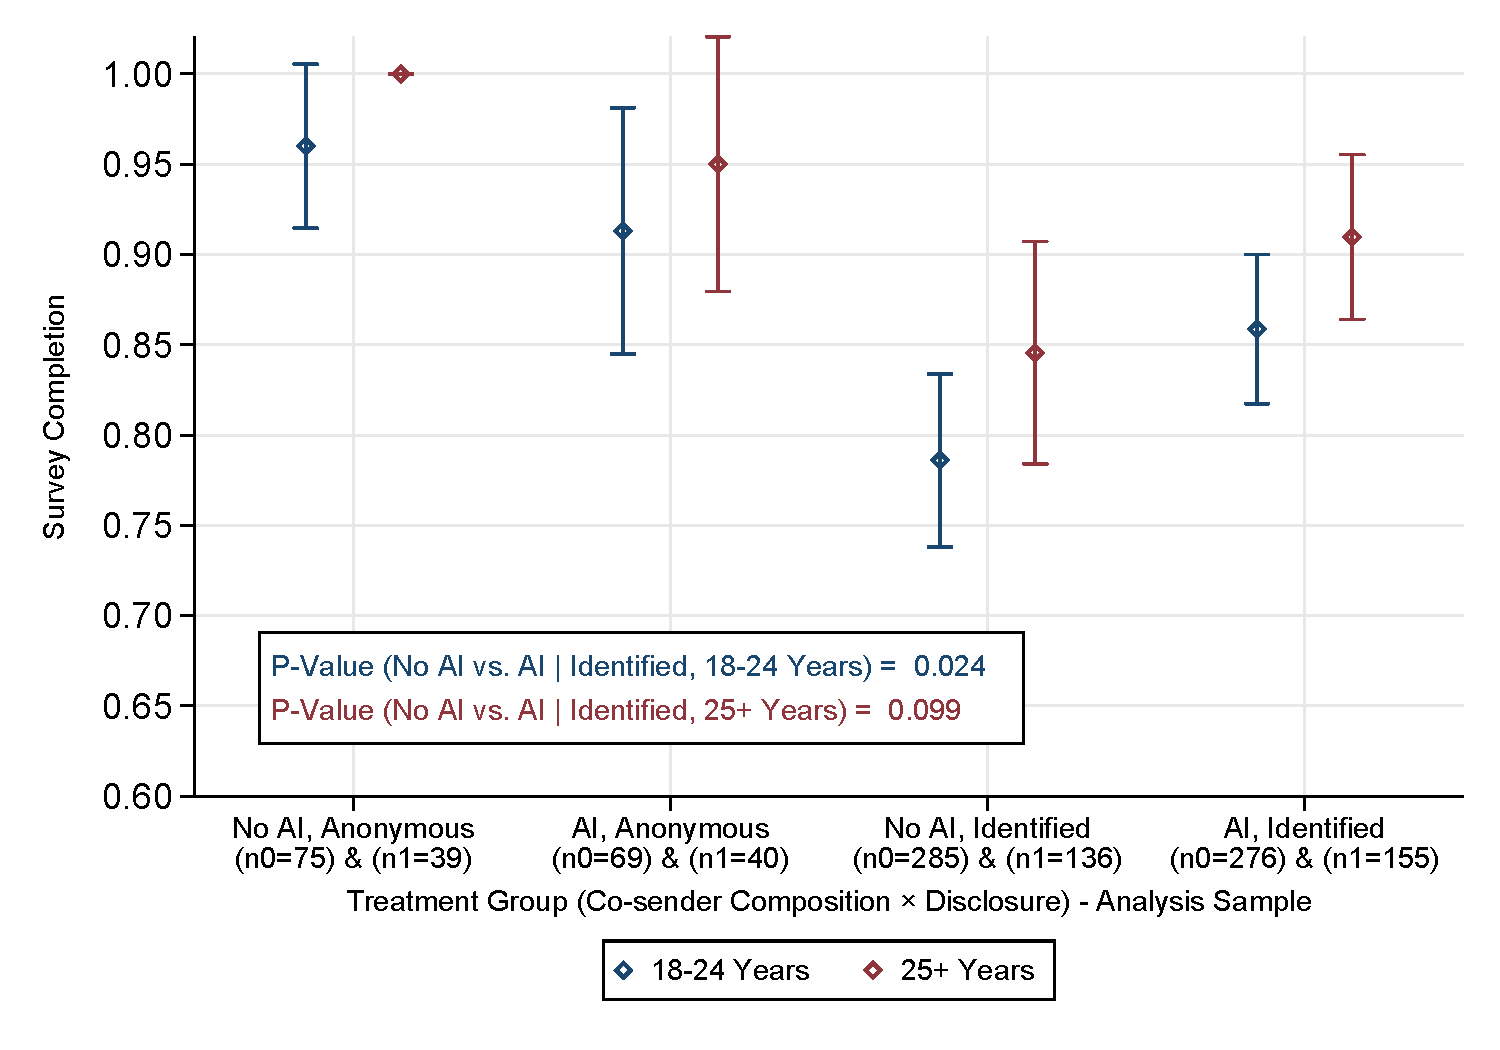
\includegraphics[width=0.9\textwidth]{ciplot_Finished_hte_AgeBinary_adult_Full_raw.pdf}
\par\end{centering}
{\small{}Notes: This figure reports treatment effects on study completion by age group. Estimates are based on respondents who passed the attention check. Error bars denote 95\% confidence intervals.}{\small\par}
\end{figure}



\begin{figure}[H]
\caption{Heterogeneity by Nationality \label{fig:nationality}}

\medskip{}

\begin{centering}
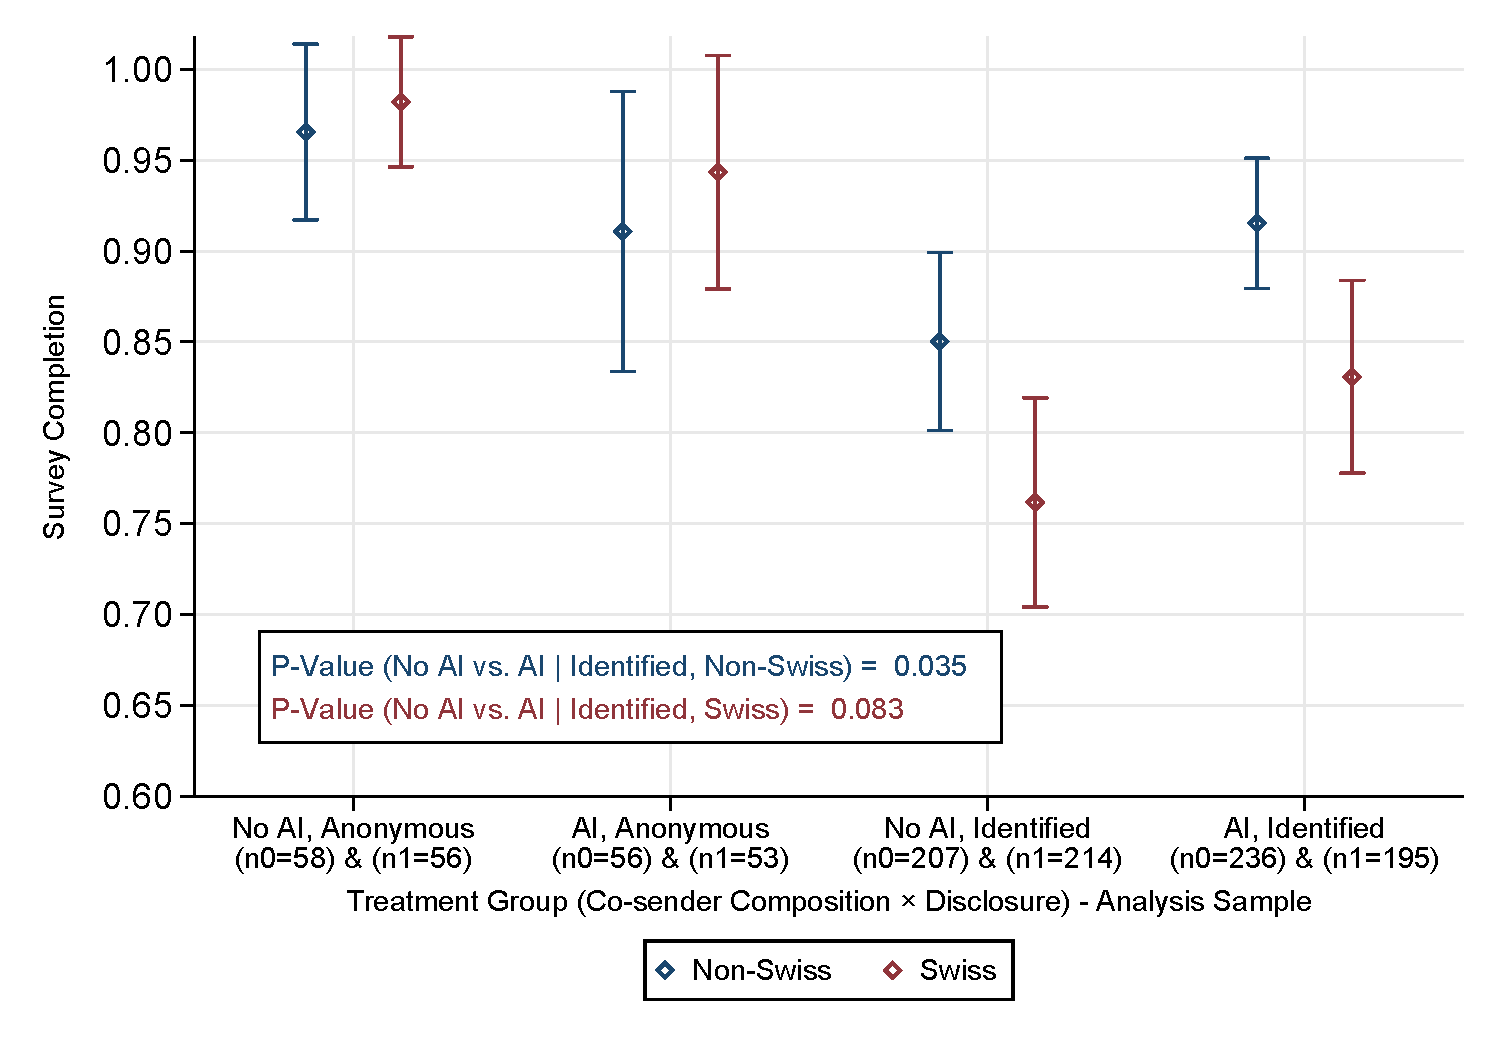
\includegraphics[width=0.9\textwidth]{ciplot_Finished_hte_Switzerland_Full_raw.pdf}
\par\end{centering}
{\small{}Notes: This figure reports treatment effects on study completion by nationality. Estimates are based on respondents who passed the attention check. Error bars denote 95\% confidence intervals.}{\small\par}
\end{figure}



\begin{figure}[H]
\caption{Heterogeneity by Gender \label{fig:gender}}

\medskip{}

\begin{centering}
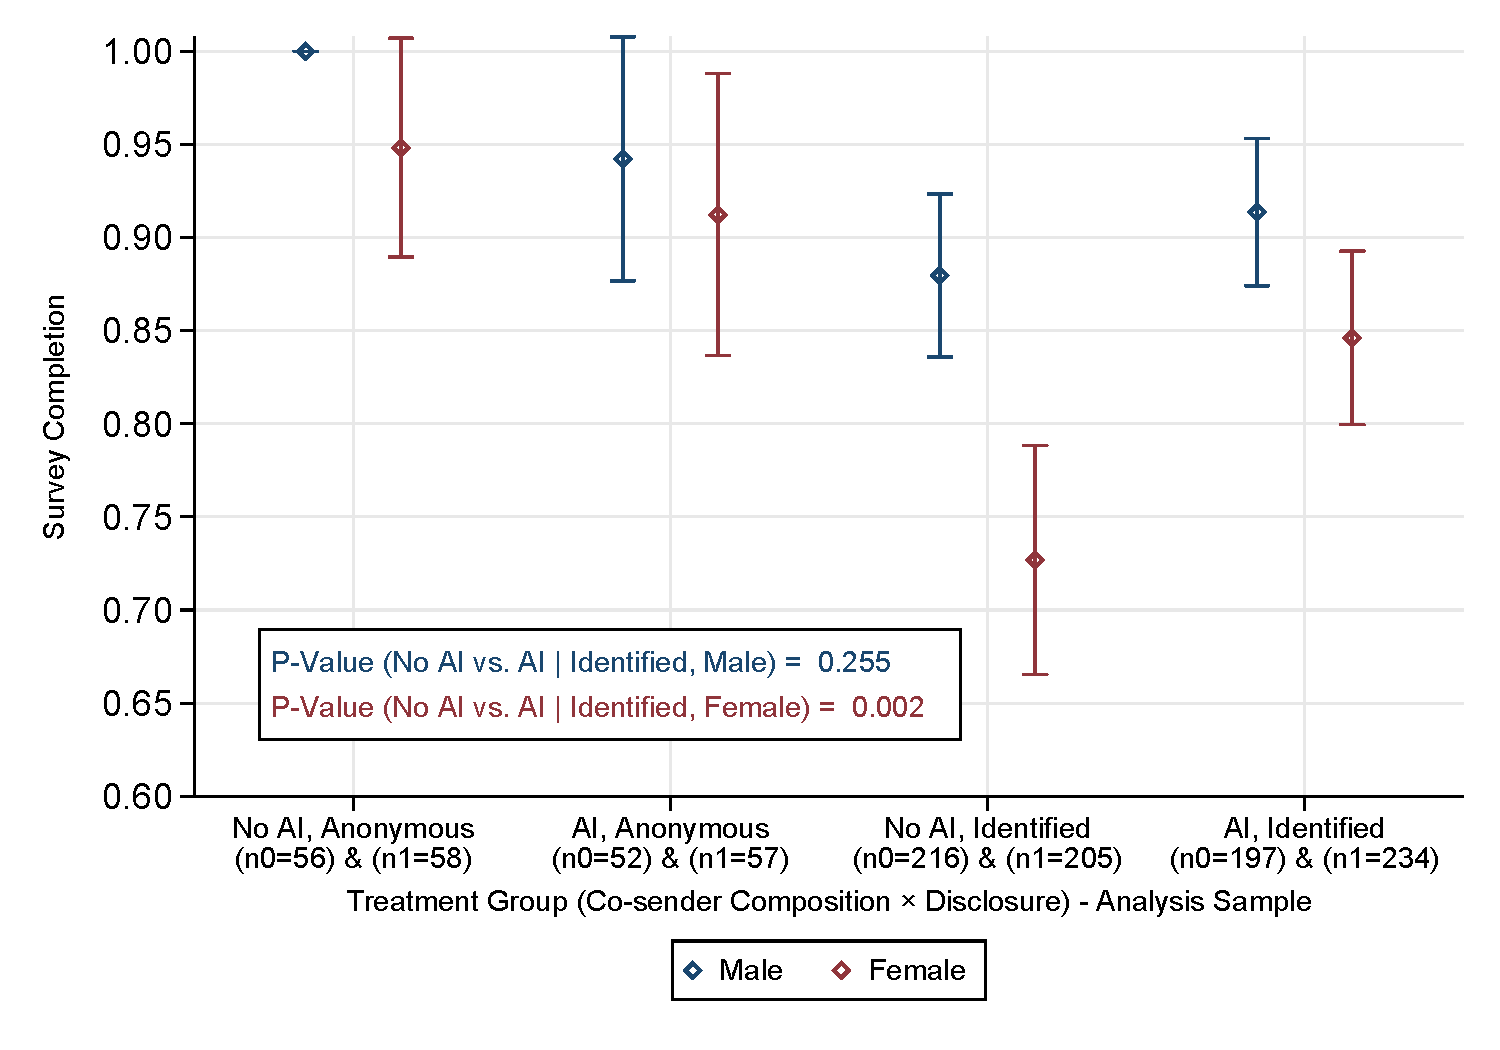
\includegraphics[width=0.9\textwidth]{ciplot_Finished_hte_Female_Full_raw.pdf}
\par\end{centering}
{\small{}Notes: This figure reports treatment effects on study completion by gender. Estimates are based on respondents who passed the attention check. Error bars denote 95\% confidence intervals.}{\small\par}
\end{figure}


\clearpage

\subsection{Deviations from the Pre-analysis Plan}\label{sec:pap}

The pre-analysis plan specifies the experimental design, outcome variables, estimating equations, and moderators. The primary pre-specified outcomes are the effort participants put into writing the post and their willingness to publicly disclose the content. In particular, after submitting their message participants are given the opportunity to pay to have their response removed from the database of posts that may be shown in a follow-up study. We use a Becker–DeGroot–Marschak (BDM) mechanism (\citealp{becker1964measuring}) to elicit an incentive-compatible valuation of how much participants are willing to pay to keep their post from being shared.\footnote{In the BDM mechanism, we randomly assigned a computer offer of zero to 99\% of participants, ensuring that nearly all posts were removed from the database at no cost. The remaining 1\% received a randomized positive offer. For the small number of posts that remained in the database, they were reviewed by a member of the research team following the procedure described to participants.} This design choice reflects our ex ante intent to measure disclosure behavior directly, rather than relying solely on stated preferences or hypothetical responses.

Our main deviation from the pre-analysis plan is that we use survey completion as the primary outcome. The PAP specified outcomes measured after the writing task, including effort and willingness to pay to remove the post. In the experiment, however, we observed substantial attrition precisely at the writing task, despite very low attrition earlier in the survey. A nontrivial share of participants chose to exit at this stage, thereby forgoing the CHF 10 participation payment, rather than proceed with the writing task. As a result, post-level outcomes are observed only conditional on completion. We therefore focus on survey completion as the primary outcome, interpreting it as a revealed-preference measure of participation in opinion sharing and content production. We additionally analyze primary writing-task outcomes, coding them as zero for participants who exited prior to completing the task, and show that the qualitative patterns are consistent across measures.

The pre-specified primary outcomes are time spent on the post, message length, and willingness to pay to remove the post. Because willingness to pay is elicited after the writing task, this outcome is subject to differential attrition. We report this result in Appendix Figure~\ref{fig:wtp} for completeness.


The fact that a nontrivial share of participants chose to exit the survey and forgo a CHF 10 payment precisely at the writing task suggests that the treatment manipulations affected a high-stakes behavioral margin not anticipated at the design stage. While this limits what can be learned from the pre-specified conditional outcomes, survey completion itself provides a revealed-preference measure of willingness to participate in content production that is directly relevant to the model's predictions.


\begin{figure}[H]
\caption{Willingness to Pay to Remove Post \label{fig:wtp}}
\medskip{}
\begin{centering}
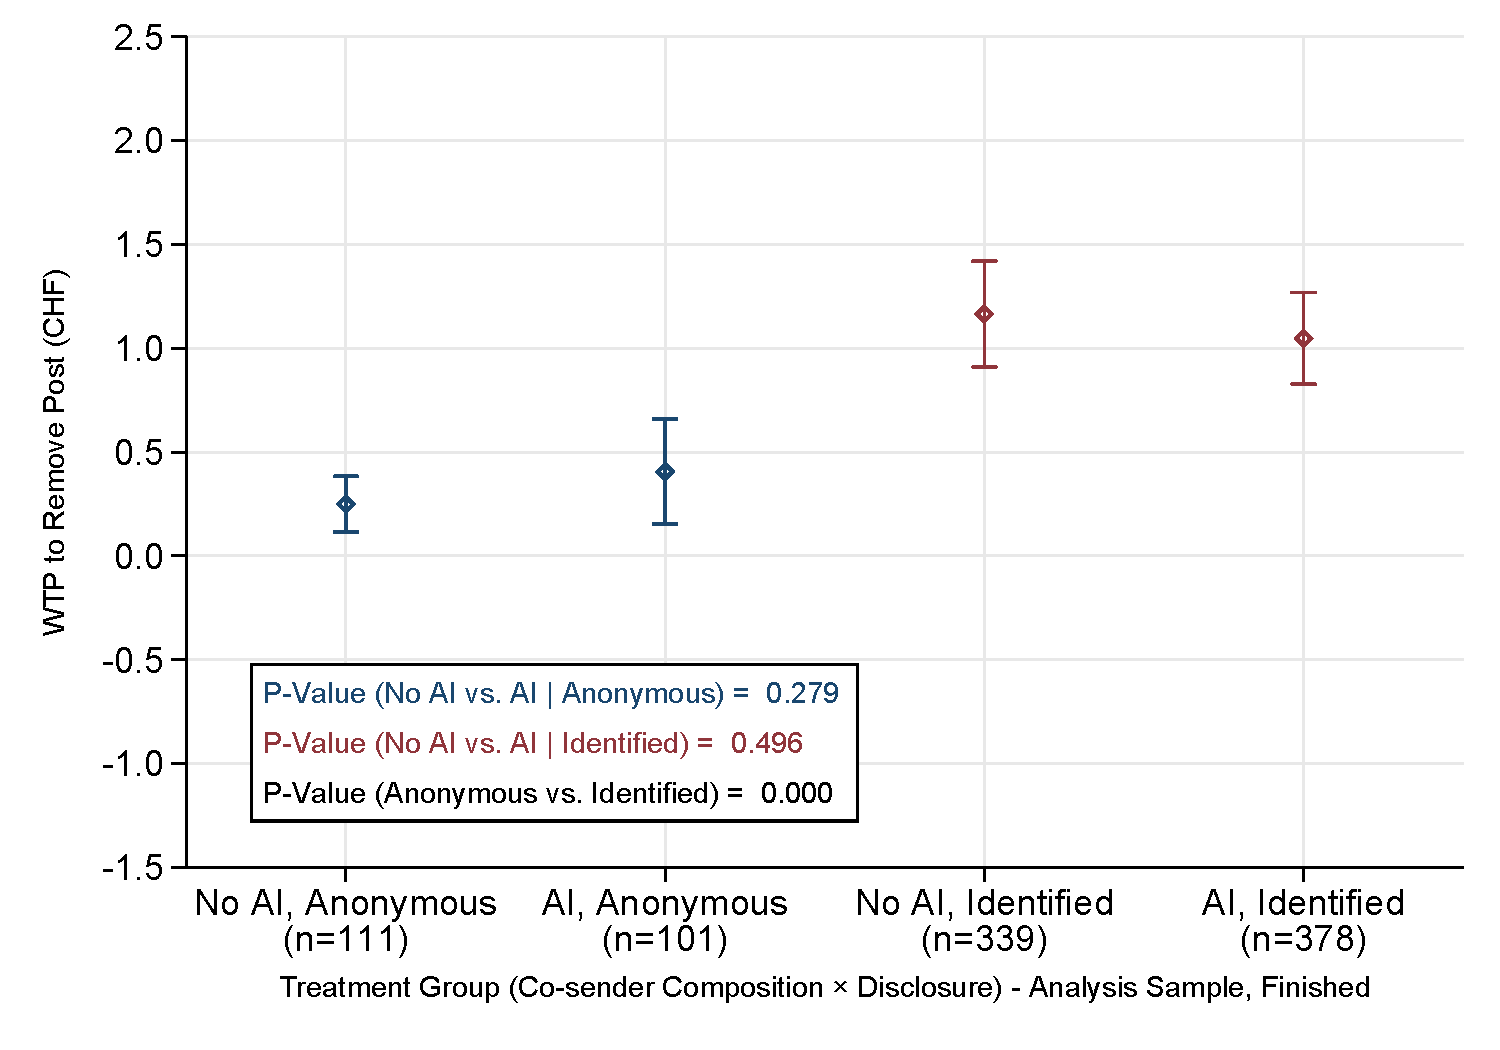
\includegraphics[width=0.7\textwidth]{ciplot_WTP_Full_raw_finished.pdf}
\par\end{centering}
{\small{}Notes: This figure reports treatment effects on willingness to pay to remove a post in CHF. Estimates are based on respondents who passed the attention check and completed the survey. Error bars denote 95\% confidence intervals.}{\small\par}
\end{figure}




\clearpage 

\subsection{Survey Instrument \label{app:SurveyInstrument}}

%% -------------------------------------------------------
%% SCREENING
%% -------------------------------------------------------
\vspace{12pt}
\emph{Screening}

\begin{enumerate}
\item What is your age? \emph{[number entry box]}
\item What gender do you most strongly identify with? \emph{[Male / Female / Other or Non-binary]}
\item Which university are you at? \emph{[ETH / UZH / Other]}
\item What is your anticipated year of graduation?\\
\emph{[2024 or earlier (already graduated) / 2025 / 2026 / 2027 / 2028 or after]}
\end{enumerate}

\emph{[Continue if age $\geq$ 18 and GradYear $\geq$ 2025 and University $\neq$ Other.]}

%% -------------------------------------------------------
%% INTRODUCTION
%% -------------------------------------------------------
\vspace{12pt}
\emph{Introduction}

Congrats! You are qualified to participate!

We are a \textbf{non-partisan group of researchers} who study public opinion in Europe and the US. \textbf{Participants like you are crucial to the study.} It is essential that you \textbf{read each question carefully and answer honestly.} You might not agree with all the information presented and that is perfectly fine. Our survey will give you an opportunity to express your views. This survey takes around 20 minutes (on average) to complete.

%% -------------------------------------------------------
%% CONSENT AND ADDITIONAL DEMOGRAPHICS
%% -------------------------------------------------------
\vspace{12pt}
\emph{Consent and Additional Demographics}

Thanks for agreeing to participate! We value your opinions and are interested in hearing what you think.

\begin{enumerate}
\item What is your first name? \emph{[text entry box]}
\item What is your country of origin? \emph{[dropdown menu]}
\item What level of education are you currently pursuing?\\
\emph{[Bachelor's degree / Master's degree / PhD / Other]}
\item \emph{[If ETH]} What faculty do you study in?\\
\emph{[Architecture and Civil Engineering / Engineering Sciences / Natural Sciences and Mathematics / System-oriented Natural Sciences / Management and Social Sciences]}
\item \emph{[If UZH]} What faculty do you study in?\\
\emph{[Faculty of Theology / Faculty of Law / Faculty of Business, Economics, and Informatics / Faculty of Medicine / Vetsuisse Faculty / Faculty of Arts and Social Sciences / Faculty of Science]}
\end{enumerate}

%% -------------------------------------------------------
%% POLITICAL AND CLIMATE OPINIONS
%% -------------------------------------------------------
\vspace{12pt}
\emph{Political and Climate Opinions}

\begin{enumerate}
\item Which party did you vote for in the last election?\\
\emph{[I did not vote in the last election / Swiss People's Party / Social Democratic Party / FDP.~The Liberals / Green Party / The Centre / Green Liberal Party / Evangelical People's Party / Federal Democratic Union / Ticino League / Swiss Labour Party / Small leftist parties (Solidarity, Together on the Left, Alternative Left) / Center Left-CSP (former Christian Social Party) / Liberal-Democratic Party (Basel) / Movement of the Citizens of French-speaking Switzerland / Pirate Party Switzerland / Mixed vote / Other]}
\item How worried are you about climate change?\\
\emph{[Not at all worried / Not very worried / Moderately worried / Very worried / Extremely worried]}
\item To what extent do you feel a personal responsibility to try to reduce climate change?\\
\emph{[Not at all responsible / Slightly responsible / Moderately responsible / Very responsible / Extremely responsible]}
\item What do you think are the most serious consequences of climate change for Europe and the world? \emph{[open text]}
\end{enumerate}

%% -------------------------------------------------------
%% SOCIAL MEDIA USE
%% -------------------------------------------------------
\vspace{12pt}
\emph{Social Media Use}

\begin{enumerate}
\item Which of the following social media platforms do you use? \emph{[multiple answer]}\\
\emph{[Facebook (excluding Facebook Messenger) / Instagram / Snapchat / TikTok / X / Twitter / BlueSky / LinkedIn / Reddit / YouTube / Other / I don't use social media]}
\item \emph{[If uses social media]} How important is it to you that other people perceive you positively on social media?\\
\emph{[Not important at all / Slightly important / Moderately important / Very important / Extremely important]}
\end{enumerate}

%% -------------------------------------------------------
%% PROSOCIAL BEHAVIOR
%% -------------------------------------------------------
\vspace{12pt}
\emph{Prosocial Behavior}

\begin{enumerate}
\item As part of completing this survey, you are automatically enrolled in a lottery to win CHF 100. Would you be willing to donate part of your winnings to an organization working on issues of climate change? If you win, you will receive CHF 100 minus the amount of your donation. We will directly donate your desired amount to the organization you specify, so no further action is required on your part.\\
Enter the amount you would like to donate, if any. \emph{[number entry box]}
\item \emph{[If donation $>$ 0]} Which organization would you like your donation to support? \emph{[text entry box]}
\end{enumerate}

%% -------------------------------------------------------
%% BOT AND AI OPINIONS
%% -------------------------------------------------------
\vspace{12pt}
\emph{Bot and AI Opinions}

In this study, we are interested in your views about two types of ``bots'' -- that is, automated programs designed to perform tasks or engage in conversations with humans.

The first type, known as `\textbf{rule-based bots},' operate on a set of predefined rules and responses. They are programmed to recognize specific commands and provide corresponding answers. These bots are often found in customer service chat functions, where they can efficiently handle routine inquiries without human intervention. \textbf{Rule-based bots have a specific, limited functionality, and it is easy to distinguish them from humans.}

The second type represents a more advanced form of technology: `\textbf{Conversational Generative AI (Gen-AI) bots}.' These bots leverage artificial intelligence to perform complex problem-solving tasks and to generate responses that mimic human conversation. Unlike their rule-based counterparts, Gen-AI bots can understand and respond to a wider range of queries with greater nuance, variability, and creativity. They learn from interactions to improve their responses, making them more adaptable and capable of handling deep conversations. As a result, \textbf{Gen-AI bots are difficult to distinguish from humans.}

\begin{enumerate}
\item How familiar are you with ChatGPT and other Gen-AI bots?\\
\emph{[I am very familiar and use them frequently / I am somewhat familiar and use them occasionally / I am somewhat familiar but rarely use them / I am aware of them but do not use them / I am not familiar with them at all]}
\item When seeking customer service or support, what are your preferences for interacting with humans, traditional rule-based bots, or conversational Gen-AI bots?\\
\emph{[Matrix; rows: Humans / Traditional rule-based bots / Conversational Gen-AI bots; 5-point scale: 1 (Strongly Prefer Not) -- 5 (Strongly Prefer)]}
\item On social media, what are your preferences for interacting with humans, traditional rule-based bots, or conversational Gen-AI bots?\\
\emph{[Matrix; rows: Humans / Traditional rule-based bots / Conversational Gen-AI bots; 5-point scale: 1 (Strongly Prefer Not) -- 5 (Strongly Prefer)]}
\end{enumerate}

Here is a potential social media post:

\begin{quote}
\emph{Some of us start closer to the finish line than others. Some individuals need a boost to get their lives back on track. It feels good to give when you are fortunate to have enough. Let's all do our part and donate to things that matter to us.}
\end{quote}

\begin{enumerate}
\item How would you react if you saw this post on your social media timeline?\\
\emph{[Like / Dislike / I would not react to this post]}
\end{enumerate}

The post you just reacted to is written by a human.

For your information, here is a potential social media post, written by a \textbf{GPT-powered Gen-AI bot}:

\begin{quote}
\emph{Many people face obstacles that are too big to tackle alone. Donating provides essential support to those who need a little extra help to overcome challenges. When we contribute to causes close to our hearts, we create a ripple of positive change in the world. Let's all pitch in and make a difference where we can.}
\end{quote}

Here is another potential social media post, written by a \textbf{rule-based bot}:

\begin{quote}
\emph{I am a bot programmed to remind people that donating is important because it helps those in need.}
\end{quote}

\begin{enumerate}
\item How effective do you think Gen-AI bots are at producing persuasive messages?\\
\emph{[Not at all effective / Slightly effective / Moderately effective / Very effective / Extremely effective]}
\end{enumerate}

In an earlier question, you wrote:

\emph{[insert answer to: What do you think are the most serious consequences of climate change for Europe and the world?]}

\begin{enumerate}
\item How different do you think your writing feels compared to something generated by AI?\\
\emph{[Not at all different / Slightly different / Moderately different / Very different / Extremely different; answer order randomized]}
\end{enumerate}

%% -------------------------------------------------------
%% READING TASKS
%% -------------------------------------------------------
\vspace{12pt}
\emph{Reading Tasks}

In the next few questions, you will read and respond to posts that may have been written by humans, traditional rule-based bots, or conversational Gen-AI bots. Please note that all posts written by humans were created without any AI assistance.

Here is a potential social media post, drawn from a pool of four posts from 4 climate-conscious humans:

\emph{[One of the following posts was randomly drawn and shown to the participant.]}

\begin{quote}
\emph{Addressing climate change is an important global issue, and it is great to see countries starting to collaborate on it. We are doing our part to help with it, too. However, while addressing climate change is important, we have other important local issues to focus on. Improving healthcare, reducing inflation and financing retirement provisions deserve our attention, too.}
\end{quote}

\begin{quote}
\emph{If we are in a spot to contribute to charity, the impacts we make can last a lifetime and impact generations to come. As of now, addressing climate change is the most important thing any of us could do. If we are in a place to donate, putting our money towards charities that help take care of the planet will impact future generations of children and animals.}
\end{quote}

\begin{enumerate}
\item How would you react if you saw this post on your social media timeline?\\
\emph{[Like / Dislike / I would not react to this post]}
\item What is your best guess for who wrote this text?\\
\emph{[Human / Traditional rule-based bot / Conversational Gen-AI bot]}
\end{enumerate}

Here is a potential social media post, drawn from a pool of four posts from 1 climate-conscious human, and 3 GPT-powered Gen-AI bots:

\begin{enumerate}
\item How would you react if you saw this post on your social media timeline?\\
\emph{[Like / Dislike / I would not react to this post]}
\item What is your best guess for who wrote this text?\\
\emph{[Human / Traditional rule-based bot / Conversational Gen-AI bot]}
\end{enumerate}

%% -------------------------------------------------------
%% ATTENTION CHECK
%% -------------------------------------------------------
\vspace{12pt}
\emph{Attention Check}

To ensure the validity of our research, it's important that you thoroughly read and understand the directions provided. Your comprehension directly affects the integrity of the data we collect. So, in order to demonstrate that you have read the instructions, please ignore the next question, and simply write ``I read the instructions'' in the box below. Thank you very much.

\begin{enumerate}
\item Please describe how you think AI is impacting your daily life. \emph{[open text]}
\end{enumerate}

%% -------------------------------------------------------
%% INSTAGRAM HANDLE
%% -------------------------------------------------------
\vspace{12pt}
\emph{Instagram Handle Collection}

\emph{[Shown only to participants who indicated Instagram use.]}

\begin{enumerate}
\item We would like to offer you some additional payments. If you provide a valid Instagram handle, you will receive an additional entry into a CHF 100 lottery. We will use the handle you provide to verify your account and check its authenticity before we send out payments. Are you interested in this offer? \emph{[Yes / No]}
\item \emph{[If interested]} What is your Instagram handle? Please provide the handle of the account that you use the most. \emph{[text entry box; validated to alphanumeric characters, periods, and underscores, up to 30 characters]}
\end{enumerate}


%% -------------------------------------------------------
%% WRITING TASK
%% -------------------------------------------------------
\vspace{12pt}
\emph{Writing Task}

We have a writing task for you. For this task, we invite you to write a post on the following topic:

\textbf{How can you and other students in Zurich contribute to combating climate change in their daily lives?}

A previous survey found that 96\% of students believe climate change is a global threat.

Your response will be added to a database of \emph{[student-written posts / 75\% AI-generated posts and 25\% student-written posts]}. We will use this database in a follow-up survey with ETH/UZH students, where each post has a 1 in 20 chance of being randomly selected. In this follow-up survey, \textbf{recipients will carefully read your post and share their opinion about both you and your post}. They will be informed that the post is drawn from a database of \emph{[student-written posts / 75\% AI-generated posts and 25\% student-written posts]}.

Along with your post, \textbf{we will share that the post is written by \emph{[identified: Name (@InstagramHandle) / anonymous: a student]} from [University Name] ([Major], [Year])}.

\begin{enumerate}
\item To make sure everything is clear, please answer the following question: If there are 100 posts in the database, how many of them are AI-generated? \emph{[0 / 25 / 50 / 75 / 100]}
\end{enumerate}

\emph{[Participants received feedback on whether their answer was correct before proceeding.]}

\begin{enumerate}
\item Write your post in the space below. You may consider sharing personal experiences and stories to make your response more engaging, but this is entirely optional. \emph{[text entry box; tab-switching and copy-paste tracking enabled]}
\end{enumerate}

%% -------------------------------------------------------
%% WILLINGNESS TO PAY
%% -------------------------------------------------------
\vspace{12pt}
\emph{Willingness to Pay to Withdraw Post}

For the writing task, you wrote:

\emph{[insert text]}

Your participation payment for this survey is CHF 10. Before we wrap up, we'd like to understand how you feel about having your post remain in our database so that it can be shared with other students. You will now have the option to give up a part of your CHF 10 to guarantee that the post does not appear in the database and will not be shared with anyone else.

Below, we ask you the maximum amount (out of your CHF 10) you'd be willing to pay to remove your post from the database.

\begin{itemize}
\item If you want your post removed (i.e., you do not want to share it), you will be willing to give up at least a small part of your CHF 10 so the post does not appear in the database.
\item If you want your post to remain (i.e., you want it shared with other students) or you are indifferent, you will not be willing to give up any money for the post to not appear in the database.
\end{itemize}

Before you began the writing tasks, the computer randomly generated an offer for you between 0 and 10.

\begin{itemize}
\item If the amount you state in your answer is equal to or greater than the computer's offer, your post will be removed and you will pay the offer amount from your CHF 10 participation payment.
\item If the amount you state in your answer is less than the computer's offer, your post will remain in the database, and you will keep the full CHF 10.
\end{itemize}

The offer is random, and \textbf{it is in your best interest to answer carefully and honestly} to ensure you get the outcome you want.

\begin{enumerate}
\item What is the maximum amount (out of your CHF 10 participation payment) you would be willing to pay to remove your post from the database?\\
\emph{[Slider from 0 to 10 CHF in 0.25 increments; initialized at 5; participants prompted to engage with the slider if left unmoved]}
\end{enumerate}

%% -------------------------------------------------------
%% PERCEPTIONS AND MECHANISMS
%% -------------------------------------------------------
\vspace{12pt}
\emph{Perceptions and Mechanisms}

You wrote:

\emph{[insert text]}

\begin{enumerate}
\item Compared to ETH/UZH students, do you think Gen-AI bots are more or less effective at writing posts that attract likes from other students in Zurich?\\
\emph{[More effective / Equally effective / Less effective / Unsure]}
\end{enumerate}

You wrote:

\emph{[insert text]}

\begin{enumerate}
\item If the audience reads your post, how likely do you think they will believe it's AI-generated?\\
\emph{[Very unlikely / Somewhat unlikely / Neutral / Somewhat likely / Very likely]}
\end{enumerate}

You wrote:

\emph{[insert text]}

\begin{enumerate}
\item How important is it to you that the audience perceives you positively?\\
\emph{[Not important at all / Slightly important / Moderately important / Very important / Extremely important]}
\end{enumerate}

You wrote:

\emph{[insert text]}

\begin{enumerate}
\item How engaged do you think you'll seem to the audience in issues of climate change?\\
\emph{[Very engaged / Somewhat engaged / Neutral / Slightly disengaged / Very disengaged]}
\end{enumerate}

%% -------------------------------------------------------
%% WTP LONG
%% -------------------------------------------------------
\vspace{12pt}
\emph{Willingness to Pay Explanation}

You wrote:

\emph{[insert text]}

\begin{enumerate}
\item \emph{[If WTP $>$ 0]} Could you explain why you want to pay to remove your post? What factors influenced your decision? \emph{[open text]}
\item \emph{[If WTP $=$ 0]} Could you explain why you do not want to pay to remove your post? What factors influenced your decision? \emph{[open text]}
\end{enumerate}

%% -------------------------------------------------------
%% STUDY PURPOSE
%% -------------------------------------------------------
\vspace{12pt}
\emph{Study Purpose}

\begin{enumerate}
\item If you had to guess, what would you say our research project is about? \emph{[open text]}
\end{enumerate}

%% -------------------------------------------------------
%% FINAL COMMENTS AND DEBRIEF
%% -------------------------------------------------------
\vspace{12pt}
\emph{Final Comments}

Thank you! We really appreciate you for participating in this research! On the next and final page, we will share insights about the purpose and significance of this study.

\begin{enumerate}
\item Please share any additional feedback or comments. \emph{[open text]}
\end{enumerate}

\textit{[Participants then received a full debrief explaining the purpose and significance of the study.]}

\end{document}
